\documentclass[11pt, oneside]{memoir}   	% use "amsart" instead of "article" for AMSLaTeX format
\usepackage{geometry}                		% See geometry.pdf to learn the layout options. There are lots.
\geometry{letterpaper}                   		% ... or a4paper or a5paper or ...
\usepackage{graphicx}
\usepackage{color}
\usepackage[dvipsnames]{xcolor}
\usepackage{enumerate}
\usepackage{amssymb}
\usepackage{footnote}
\usepackage{enumerate}
\usepackage{eucal}
\usepackage{amsmath}
\usepackage{braket}
\usepackage[utf8]{inputenc}
\usepackage[english]{babel}
\usepackage{hyperref}
\usepackage{xspace}

\hypersetup{
    colorlinks,
    citecolor=red,
    filecolor=red,
    linkcolor=red,
    urlcolor=red
}

\setcounter{tocdepth}{3}
\setcounter{secnumdepth}{3}

\newcommand{\zeronu}{0\nu\beta\beta}
\newcommand{\twonu}{2\nu\beta\beta}
\newcommand{\Tl}{$^{208}$Tl}
\newcommand{\Co}{$^{60}$Co}
\newcommand{\Pb}{$^{208}$Pb}
\newcommand{\Bi}{$^{214}$Bi}
\newcommand{\Qbb}{Q_{\beta\beta}}
\newcommand{\Bckunit}{\text{counts.keV}^{-1}\text{.kg}^{-1}\text{.y}^{-1}}
\newcommand{\Tbeta}{T_{1/2}^{0\nu}}
\newcommand{\mbb}{m_{\beta\beta}}



\title{Searching for the $\zeronu$ decay with the SuperNEMO demonstrator}

\begin{document}
\maketitle
\pagebreak
\tableofcontents

%% \chapter*{Introduction}
\label{ch:intro}
\addcontentsline{toc}{chapter}{Introduction}

It is always interesting to take a historical approach when talking about a scientific discovery. This allows us to put into perspective knowledge that is now considered to have been acquired.

The Standard Model of Elementary Particle Physics attempts to describe the world around us on scales that were inconceivable two centuries ago.
A little over a hundred years ago, Henri Becquerel discovered what we today call radioactivity, with the observation of $\beta$ decay.
This historical discovery was nevertheless accompanied by profound questioning, since the $\beta$ particle emitted during this decay, which turned out to be an electron, only carries away part of the available energy for the reaction.
This observation was contrary to the first principle of thermodynamics on the energy conservation, and some scientists postulated that this fundamental law was being violated.
It took 35 years for an eminent scientist by the name of Wolfgang Pauli to propose the existence of the \emph{neutrino} ($\nu$) - for small neutron in Italian - as a solution to the problem of missing energy.
Three years later Enrico Fermi laid the foundations for the first mathematical formulation of what is today the Lagrangian of weak interaction.
It was another 25 years, 60 years after the discovery of $\beta$ radioactivity, before the neutrino was experimentally observed by Clyde Cowan and Frederick Reines.
The neutrino adventure had only just begun.

Why is this particle, although abundantly produced in the sun in the atmosphere and in the earth, so difficult to detect?
It is because it interacts very little with the matter - electrons and quarks - that constitutes us, being sensitive only to the weak interaction (of short range), and to the gravitational force (very weakly since the mass of the neutrino is extremely low, so much that it was believed massless for a long time).

In the current model of particle physics, neutrinos are actually described as massless.
It was Bruno Pontecorvo who proposed in 1957 that neutrinos could oscillate between their different mass states, based on the already known model of oscillation of neutral kaons.
To be valid, this model then presupposed that neutrinos had a non-zero mass.
It was the SuperKamiokande experiment that first observed this phenomenon in 1998, demonstrating that at least two of the three neutrino flavours have a non-zero mass.
The Standard Model of particle physics is then no longer sufficient to account for this particle properties, opening the way to physics beyond the Standard Model.

It now remains to be discovered how this particle acquires its mass.
Indeed, having a neutral charge under the three fundamental interactions described by the Standard Model, two mass generation mechanisms are foreseeable.
The first is to assume that, like all other fermions, the neutrino obtains its mass through the Higgs mechanism, leading irremediably to the assumption of the existence of a sterile neutrino.
The second, proposed by Ettore Majorana, assumes that the neutrino is its own antiparticle, giving the neutrino its mass with the addition in the Lagrangian of the Majorana mass term.
If this assertion is the one that applies to neutrinos, then a disintegration, prohibited in the Standard Model, is possible.
It is called \emph{neutrinoless double beta decay} ($\zeronu$), to contrast with the \emph{two neutrinos double beta decay} ($\twonu$) allowed by the Standard Model and already observed for several isotopes.
In the former disintegration, two simple $\beta$ decays take place simultaneously in the same nucleus, in which the two neutrinos are absorbed, allowing the total energy of the reaction to be distributed between the two exiting electrons.
For reasons that are detailed in the first chapter of this manuscript, which deals with the phenomenology of the neutrino, this disintegration is only possible if the neutrino is a Majorana particle.

Several experiments, also described in the first chapter, are dedicated to the search for this disintegration which, if it exists, is expected to be extremely rare.
%%Its observation would prove the neutrino is a Majorana particle.
The SuperNEMO experiment, on which I conducted my PhD, is one of them.
Successor of the NEMO experiments, it uses a unique combination of technologies, described in detail in the second chapter, allowing to trace the path of the electrons resulting from double $\beta$ disintegrations -with a wire chamber-, and also to measure their energies - with a segmented electromagnetic calorimeter.

These generation of experiments differ from one another in the technology they use, and also in the sensitivity they can achieve in the search for this decay.
Within the framework of this PhD, I carried out a sensitivity study of this experiment presented in the third chapter, determining the influence that several characteristics of the detector can have on it.

All these experiments are designed to observe, should this process exist, an extremely rare physical event.
They are thus constrained to focus on the background which may disturb the measurement and have a non-negligible impact on their sensitivity to this disintegration.
In this perspective, the fourth chapter presents a new technique to identify the events resulting from one of the main background for this experiment, which is the natural disintegration of an isotope from the uranium 238 decay chain, found in the detector's components.
To effectively reject this background, I also study the impact on the sensitivity of the accuracy with which we measure the arrival time of particles in the calorimeter.
To complete this theoretical analysis based on simulations of the detector, the fifth chapter gives an overview of the data taken at Modane with the SuperNEMO calorimeter and of the analysis aiming to characterise the time resolution for a large part of the optical modules.

When I joined the LAL team at Orsay (now IJCLab) as a PhD student, SuperNEMO was already largely built in the Modane underground laboratory.
I had the opportunity to actively participate in the completion of its assembly, as well as in the analyses of the first commissioning data described in the last chapter, thus completing the experimental knowledge acquired during this PhD.

%% \chapter{Phenomenology of particle physics}
\section{The Standard Model of particle physics}
\subsection{Bosons}
\subsection{Fermions}
\subsection{$\twonu$ decay}
\subsection{Where the Standard Model ends}
\section{Going beyond the Standard Model with neutrinos}
\subsection{Neutrino flavors and oscillations}
\subsection{Neutrino masses and nature}
\label{subsec:nu_mass_nature}
\subsection{Other searches beyond the Standard Model with neutrinos}

%% \include{0nubbexperiments/0nubbexperiments}
%% \chapter{The SuperNemo demonstrator}
\label{ch:detector}

\section{The SuperNemo demonstrator}
\subsection{Comparison with Nemo$3$ experiment}
\subsection{Expermimental design}
\subsection{Sources}
\subsection{Tracker}
\subsection{Calorimeter}
\label{subsec:SN_calo}



\subsubsection{Scintillator}





\subsubsection{Photomultiplier}
\label{sec:calorimeter}
\subsection{Calibration systems}
\subsection{Control Monitoring system}
\subsection{Electronics}

\section{The backgroung of SuperNEMO}
\label{sec:SNbkg}
\subsection{Internal background}
\label{subsec:SNbkg_internal}

Trace quantities of naturally-occurring radioactive isotopes can occasionally produce two-electron events and thus can mimic $\beta\beta$-decay events.
The largest contributions come from isotopes of decay chains of $^{238}$U, $^{232}$Th and $^{40}$K, which disintegration occur inside the source foils, as well as inside the tracking volume.

Décire la contamination mesurée des sources, et du radon dans la partie suivante

\subsection{External background}
Radon:\\
Radon is a noble gas which occurs as an indirect decay product of uranium and thorium.
Due to its chemical properties, radon has a long diffusion length in solids, making it difficult to remove.
Radon contaminations inside the tracker volume is a major background to the rare event experiments such as SuperNEMO.
Simulations show that, to achieve the designed sensitivity, the level of radon must not exceed $0.15$ mBq/m$^{3}$ since its decay daughter \Bi, $\Qbb= 3.2$ MeV can mimic a $\zeronu$ event.
Radon concentration measurements inside the demonstrator tracker have been performed by the SuperNEMO collaboration, revealing an activity of $0.15\pm0.02$ mBq/m$^{3}$, through the combination of an anti-radon tent and an air-flushing method.

%%Repris d'un article -> a changer:
They are outgased in the air from the rock walls of the experimental hall and can enter the detector either through tiny gaps between sectors or through gas pipe joints.
The progeny of radon and thoron produces $\gamma$-rays and $\beta$ decays accompanied by internal conversion (IC), Møller or Compton scattering.
\subsection{Background specifications}
\subsection{Measured demonstrator background levels}

\section{Magnetic field}
\label{sec:magnetic_field}

\section{The SuperNemo software}
\label{sec:SNsoftware}
\subsection{Simulation}

As described in Sec.~\ref{sec:SNsoftware} of Chapter~\ref{ch:detector}, the SuperNEMO collaboration developed its own simulation, reconstruction and analysis environment.
The Falaise software, specifically designed by and for the SuperNEMO collaboration, holds the \verb!C++! library for the event reconstruction and analysis of simulated and real data.
Especially, it contains the geometry, the detector material, the event data model, the reconstruction algorithms and the data analysis.
Finally, the SNFee software is a tool package for the configuration, control and monitoring of the SuperNEMO front-end electronics.

\subsection{Reconstruction}

%% \chapter{Analysis tools}


\subsection{Internal probability}
\label{subsec:internal_prob}
Internal probability is a mathematical tool used to quantify the probability that two particles (in this study only electrons will be considered) were emitted simultaneously and at the same location in the source foils.
The internal probability is defined from the associated internal $\chi^{2}$
\begin{equation}
  \chi^{2}_{int}=\frac{((t^{exp}_{1} - \frac{L_{1}}{\beta_{1} c}) - (t^{exp}_{2} - \frac{L_{2}}{\beta_{2} c}))^{2}}{\sigma_{tot}^{2}}\,\text{,}
  \label{eq:int_chi2}
\end{equation}
where c is the speed of light, $t^{exp}_{i}$ is the time measured in calorimeters for the particle $i$, $L_{i}$ is the reconstructed track length, and $\beta_{i}$ is defined as $\sqrt{E_{i}(E_{i} + 2m_{e})} / (E_{i} + m_{e})$, $E_{i}$ being the energy of particle $i$ and $m_{e}$ the electron mass.\\
The denominator in eq.~\ref{eq:int_chi2} is the total uncertainty defined as
\begin{equation}
  \sigma_{tot}=\sqrt{\sigma_{t}^{2}+\sigma_{\left(\frac{L}{\beta c}\right)}^{2}+\sigma_{l}^{2}}\,\text{,}
  \label{eq:sigma_tot}
\end{equation}
where the first term $\sigma^{2}_{t}=\sum_{i=1,2}\sigma^{2}_{t_{i}}$ is the uncertainty the time measurement in the calorimeters with $\sigma_{t}$ defined as
\begin{equation}
  \sigma_{t}=\sqrt{\dfrac{\tau_{\text{SC}}^{2}+\left(\dfrac{\text{FWHM}(\text{TTS})}{2\sqrt{2\ln{2}}}\right)^{2}}{\text{N}_\text{PE}}}\,\text{.}
  \label{eq:sigma_t}
\end{equation}
The second term $\sigma^{2}_{\left(\frac{L}{\beta c}\right)}=\sum_{i=1,2}\sigma^{2}_{\left(\frac{L_{i}}{\beta_{i}c}\right)}$ is the uncertainty depending on the energy of electron $i$ as
\begin{equation}
\sigma_{\left(\frac{L}{\beta c}\right)} = \biggl\lvert \dfrac{\partial t_{th}}{\partial E}  \biggr\rvert \Delta E\,\text{.}
  \label{eq:sigma_L}
\end{equation}
The third term $\sigma_{L}$ represents the typical uncertainty due to track reconstructions of particles\footnote{This value is set to $\sigma_{L}=0.03$ ns in a first approximation (see chapter -ref-).}.\\
Then the internal probability evaluate the difference between experimentally measured time and theoretical times.




\section{Simulations}
\subsection{Modifications of simulation software}
\subsection{Internal background simulations}
\subsection{$\zeronu$ simulations}

%% \chapter{Improvement of the internal Thallium-$208$ background rejection}
\label{ch:timediff}

At the end of September $2018$, the $34$ enriched-Selenium source foils were installed on the demonstrator.
At this time, the internal \Tl\ and \Bi\ activities of these sources had already been measured by the BiPo detector.
Also, the Radon concentration in the chamber was extrapolated from Radon emission measurements of the tracker components with a concentration line for an incoming gas flow of $2$~m$^{3}$/h.
We described in the previous chapter the impact of these activities on the final detector sensitivity to the $\zeronu$ decay, and set up optimised topological selections adjusted to reject the Radon background.

However, \Tl\ disintegrations in the sources also remains a troublesome background, even for $\beta\beta$ emitters with a high $\Qbb$.
Indeed, it contributes at high energies (up to $4$~MeV on the two electrons energy sum spectrum), because of the internal conversion of the $2.615$~MeV $\gamma$-ray.
In a context where the \Tl\ contamination is higher than expected inside the sources, we focus in the current chapter on rejection techniques peculiarly adapted to reject internal \Tl\ events.
We study the influence of these additional techniques on $\zeronu$ events selection, and evaluate the impact on final detector sensitivity.
Impact of the calorimeter timing performances on these techniques are also addressed in this chapter.

\section{Motivations}

In Chapters~\ref{ch:detector} and \ref{ch:sensitivity}, we presented the specifications set on the background activities, in order to reach the target limit on the $\zeronu$ process half-life of the \Se\ in $5$ years, with $100$~kg of isotope.
The Tab.~\ref{tab:real_target_act} given in Chapter~\ref{ch:detector} summarises the target \Tl, \Bi\ and \Rn\ activities, and provides a comparison with those measured by the collaboration.
The BiPo detector was capable of giving an upper limit on the \Bi\ level of ${\mathcal{A}^{\text{Bi}}<290~\mu}$Bq/kg at $90$\% CL, and future more precise measurements with SuperNEMO demonstrator will constraint this value.
The BiPo measurements also showed that the \Tl\ contamination is about $30$ times greater than expected on average.
We give in Tab.~\ref{tab:Nbkg_wBi} the number of expected background events for the measured activities (taking the upper limit for \Bi\ contamination), for the demonstrator and final detector.
\begin{table}[!h]
  \centering
  \begin{tabular}{|c|c|c|}
    \hline
    Exposure & Demonstrator & Detector  \\
    & $17.5$~kg.y & $500$~kg.y \\
    ROI (MeV) & [$2.7$;$3.3$] & [$2.6$;$2.95$] \\
    \hline\hline
    $\twonu$  & $0.383$ & $104$  \\
    \Tl  & $1.09$ & $21.2$  \\
    \Bi  & $1.42$ & $110$  \\
    \Rn  & $0.0782$ & $6.11$  \\
    \hline
  \end{tabular}
  \caption{Expected number of background events in the $2e$ topology, in optimised energy ranges for the SuperNEMO demonstrator ($17.5$~kg.y) and the final detector ($500$~kg.y exposure).
    The $\twonu$ half-life is taken as $\Ttwonu~=~9.39\times~10^{19}$~y, and the measured background activities are considered (with the upper limit for \Bi\ contamination).
    The topological selections have been optimised: \Pint$>4$\% and $|\Delta~Z|~<~80$~mm.
    ROI are optimised to maximise the $\Tbeta$ limit at $90$\% (see Chapter~\ref{ch:sensitivity}).
    \label{tab:Nbkg_wBi}}
\end{table}
With an activity fixed to the measured one, the \Tl\ background does not affect significantly the sensitivity of the demonstrator ($17.5$~kg.y exposure) as only one event is expected in the optimised [$2.7$;$3.3$]~MeV energy region, after first-order and topological cut-offs were applied.
On the other hand, this background could be harmful for the final detector ($500$~kg.y exposure), with $21$ events expected in the region of interest [$2.6$,$2.95$]~MeV.
To overcome this effect, it is interesting to set a specific method designed to reject \Tl\ events.

In the next section, we describe the specific features of the Thallium internal background.
We develop a new technique of rejection, especially designed to identify internal \Tl\ events, based on several Time-of-flight computations.

\section{The internal \Tl\ background}

As described in Chapter~\ref{ch:detector}, radioactive isotope disintegrations inside the source foils can occasionally produce two-electron events, and thus can mimic $\beta\beta$-decay events.
The \Tl, a progeny of \Th, is one of the largest contribution to the internal background.
Two electrons can be produced via a $\beta$-decay followed by a M\o{}ller scattering, $\beta$-decay to an excited state with the subsequent internal conversion, or due to Compton scattering of the de-excitation photon.

The disintegration scheme of \Tl\ isotope is presented in Fig.~\ref{fig:Tl_scheme}.
\begin{figure}[!h]
  \centering
  \includegraphics[width=13cm]{timedifference/fig_timediff/Tl_decay_scheme.pdf}
  \caption{A simplified disintegration scheme for the \Tl\ isotope.
    $81$~\% of the disintegration pass through the $294$~ps metastable energy level (orange).
    All disintegration go through the $2.615$~MeV energy level (green), where an orbital electron is ejected in $0.246$~\% of the cases through the internal conversion process.
  \label{fig:Tl_scheme}}
\end{figure}
This shows that \Tl\ always $\beta$-decays to an excited state of the \Pb\ daughter nuclei.
In more than $99$~\% of the decays, at least 2 $\gamma$'s are expected after the $\beta$ emission.
For $\zeronu$ detection of isotopes with high $\Qbb$, the most dangerous mode of $\beta\beta$-like events production comes from the internal conversion of the $2.615$ MeV-$\gamma$, resulting in one electron with an energy of $2.5$ MeV approximately and a beta-electron with a continuous spectrum between $0$ and $\sim~1.5$~MeV.
Thus \Tl\ events with a total energy greater than $2.7$~MeV can populate the region of interest.

\subsection{The internal conversion process}

An excited nucleus will practically constantly achieve a transition to a lower state by one of two processes: the emission of a $\gamma$-ray, or the ejection of one of the orbital electrons.
The latter, called \emph{internal conversion} (frequently abbreviated IC), is a second-order process, where an electron couples to a proton inside the excited nucleus.
Thus, in such a radioactive decay, the de-excitation energy of the nucleus is transferred \emph{directly} to a $j$-shell electron ($j=K,L,M...$).
A high-energy electron is therefore emitted from the atom, and carry off the energy
\begin{equation}
E_{IC} = E_{\gamma}-E_{j}\qquad (j=K,L,M...)\,,
\end{equation}
where $E_{j}$ is the binding energy of the electron in the $j$-shell, and $E_{\gamma}$ is the energy of the $\gamma$-ray.

This mechanism is possible because there is a non-zero probability of finding the electron within the nucleus, that is to say, the wave-function of the electron can penetrate the volume of the nucleus.
Consequently, due to their high nuclear penetration, electrons coming from the $1s$ state are more likely to be ejected (this transition is called $K$ internal conversion).
Although electrons coming from $2s$, $3s$ and $4s$ states ($L$, $M$ or $N$ internal conversions) have also a non-zero probability to undergo this process.
After the electron ejection, the hole in the corresponding shell is filled by an electron from a higher energy level, emitting characteristic $X$-rays, Auger electrons, or both.

For a given transition, the internal conversion coefficient of the electron in the $j$-shell, is defined by
\begin{equation}
\alpha_{j}=\frac{P_{IC, j}}{P_{\gamma}}\,,
\end{equation}
%% \begin{equation}
%% \alpha_{K}=\frac{P_{IC, K}}{P_{\gamma}}\,,
%% \end{equation}
where $P_{IC,j}$ is the $j$ conversion electron emission probability, and $P_{\gamma}$ is the $\gamma$-ray emission probability.
The total coefficient is
\begin{equation}
  \alpha_{T}=\sum_{j=K,L,M\cdots}\alpha_{j}\,.
\end{equation}
These coefficients are given in Tab.~\ref{tab:IC_prob} for the $2.615$~MeV energy level of \Tl\ isotope.
\begin{table}[!h]
  \centering
  \begin{tabular}{|c|c|c|c|c|}
    \hline
    $j$-shell & $K$ & $L$ & $M$ & Total \\
    \hline\hline
    IC coefficients (\%) & $0.1708$ & $0.0292$ & $0.00685$ & $0.246$ \\
    \hline
  \end{tabular}
  \caption{Internal conversion coefficients for the $2.615$~MeV $\gamma$-ray of the \Tl\ decay scheme.
    \label{tab:IC_prob}}
\end{table}
Therefore, in $0.246$~\% of the cases, the \Pb\ excited nucleus will undergone an internal conversion corresponding to the $2.615$~MeV energy level.


\subsection{\Tl\ disintegrations in the 2e channel}

Finally, a \Tl\ decay can present a two-electrons topology when, after the $\beta$ emission, an electron is ejected from the atom through internal conversion.
Especially, when this energy transfer corresponds to the $2.615$~MeV $\gamma$-ray, the ejected electron carry off a significant energy, depending on its initial binding energy with the nucleus.
For instance an orbital electron from the $K$-shell is ejected with an energy $E_{IC,K}=2.526$~MeV (${\alpha_{K}=0.17}$\%).
This decay is therefore likely to contribute in the region of interest for the $\zeronu$ search of \Se, or even \Nd.

%% In Fig.~\ref{fig:Emin_Emax_Tl} is presented the individual energy spectra for $2e$ topologies for \Tl\ simulations inside the source foils.
%% \begin{figure}[!h]
%%   \centering
%%   \includegraphics[width=13cm]{timedifference/fig_timediff/energy_spect_min_max_208Tl.pdf}
%%   \caption{Individual energy spectra for selected $2e$ topologies of \Tl\ decays simulated inside the source foils.
%%     Calorimeter hit of minimal energy (red) and maximal energy (blue).
%%     Spectra are arbitrarily normalised.
%%     The [$2.7$;$3.2$] ROI is represented by grey dashed lines.
%%     \label{fig:Emin_Emax_Tl}}
%% \end{figure}
%% An usual technique to reject \Tl\ background consists in distinguishing $2e$ topologies for which one of the two calorimeter hit has an energy greater than $2.7$~MeV.
%% The energy resolution of the demonstrator being improved by a factor of $\sim~2$ with respect to NEMO-$3$, this selection is efficient.
%% This cut-off allows to reject $0.61$~\% of the \Tl\ internal events, while rejecting only $0.11$~\% of $\zeronu$ events.

In the $2e$ channel, optimised topological cut-offs, based on time-of-flight computation and the distance between vertices, were presented in the previous chapter.
They are mostly efficient in rejecting the non-internal \Rn\ events.
After a brief presentation of the simulations carried out as part of this analysis, we remind and specify the internal probability computation, and present a new selection, also based on the time-of-flight computation, to reject the \Tl\ background.

%% \begin{itemize}
%% \item donner la proportion d'ev retardés avec la bank SD (simus en train de tourner)
%% \item relire et compléter cette sous-section
%% \item Avant d'entrer dans le détail préciser le principe de la réjection par temps de vol.
%%   L'électron de plus haute énergie est en retard, avec un retard en moyenne de 294 ps pour la plupart des niveaux (discuter un peu le schéma de désintégration, dans quel cas il sera en retard).
%%   Ensuite dire que tu as quantifié le pourcentage d'électrons de haute énergie en retard avec une simulation "parfaite" i.e. avec une résolution en  temps  nulle.
%%   A comparer avec le chiffre donné précédemment (issu d'une étude du schéma de désintégration.)
%% \end{itemize}


\section{Simulated demonstrator performances}

The background model used in the framework of this study has already been described in detail in the previous chapter.
Nevertheless, calorimeter performances implemented in the Falaise software have been modified in this study.
Indeed, one of the main goal is to evaluate the influence of the calorimeter timing performances on the \Tl\ background rejection.
This study was led before the commissioning phase of the calorimeter when timing performances were characterised only for few optical modules, and before their installation at Modane~\cite{HuberThesis}.
An encouraging value for the uncertainty on the calorimeter time measurement of $248.3$~ps for incoming electrons and $341.8$~ps for photons were provided for the best optical module tested (Fig.~\ref{fig:Arnaud_RMS_PM}).
\begin{figure}[!h]
  \centering
  \includegraphics[width=13cm]{timedifference/fig_timediff/Arnaud_RMS_PM.pdf}
  \caption{Time distribution of the trigger time of an optical module in the case of electrons (red) and gamma radiation (green) depositing an energy of $1$~MeV in the scintillator.
    The trigger threshold is set at $45$ mV and corresponds to an energy of $0.150$~MeV.
    Adapted from~\cite{HuberThesis}.
  \label{fig:Arnaud_RMS_PM}}
\end{figure}
In this context, before the full calorimeter calibration in Modane, we would give an overview of the influence of these performances on the \Tl\ background rejection.
To do so, signal and background simulations were performed supposing the optical modules measure perfectly the particle time-of-flights, by setting to zero the time uncertainty at the level of the calibration module in the Falaise pipeline.
I wrote a Root code allowing to degrade the precision on time measurements for it to be set by the user to the desired accuracy.

All of the simulations produced for this analysis were generated using the official Falaise pipeline, and are made available to the collaboration in the common SuperNEMO repository at the IN$2$P$3$ computing centre platform.
The same code described in the previous chapter has been used for this study, including the Particle Identification module, the module I wrote and the Root code pipeline.
An additional set of codes have been developed in order to degrade the simulated calorimeter resolution as well as to compute the analysis tools described in the following.

In the first instance we set the reasonable value of $200$~ps for the measurement uncertainty.
In Sec.~\ref{subsec:calo_sigma} the influence of this parameter on the \Tl\ rejection is provided, and we give final sensitivity results according to it in Sec.~\ref{sec:Tl_sensitivity}.


\section{Rejection of \Tl\ with a time-of-flight criterion}
\label{sec:Tl_TOF}


The internal probability, based on time-of-flight computation, quantifies the likelihood that two particles were emitted inside the source foils, from the same vertex.
Unless it is a useful tool, we would implement a new one, also based on time-of-flight, taking into account the possible delay between the two incoming electrons due to the \Pb\ metastable state.

%% Internal conversion occurs after $\beta$ or $\alpha$ radioactive decays leaving the nucleus excited.
%% Then a $\gamma$ particle is emitted and transfers its energy to an atomic electron which results in ejection of this electron from the atom.
%% The emitted electron has an energy corresponding to the energy of previously excited nucleus reduced by the electron binding energy.
%% After the internal conversion, electrons reorganise.
%% The hole in internal layer is filled by an electron from an external layer (emitting an X ray).\\
%% The probability for an atomic electron to be ejected decreases with the initial binding energy.
%% Thus, electrons from K layers have a higher probability to be converted (see Fig.~\ref{fig:Tl_IC}).

\subsection{The internal probability}

As part of the analysis pipeline, this tool is widely employed in NEMO-$3$ and SuperNEMO, for background rejection purposes.
We present it in detail in Chapter~\ref{ch:detector} and examine an example of its usefulness in Chapter~\ref{ch:sensitivity}.
Nevertheless, in the framework of this analysis we need to perform our own calculation of internal probability, after the reconstruction pipeline, because the simulations are performed for an ideal value of the optical module performances.
That is an opportunity to come back to this tool and to clarify certain points.

The calculation of the internal $\chi^{2}$ is reminded in Eq.~\eqref{eq:int_chi2_electrons}, for two detected electrons, as a function of the expected time-of-flights, $t^{\text{exp}}$, the experimentally measured time-of-flights, $t^{\text{meas}}$, as well as the total uncertainty on the time-of-flight measurement:
\begin{equation}
  \chi^{2}_{int}=\frac{((t^{\text{meas}}_{1} - t^{\text{exp}}_{1}) - (t^{\text{meas}}_{2} - t^{\text{exp}}_{2}))^{2}}{\sigma_{t_{1}}^{2}+\sigma_{t_{2}}^{2}+\sigma_{\beta_{2}}^{2}+\sigma_{\beta_{1}}^{2}+\sigma_{l_{1}}^{2}+\sigma_{l_{2}}^{2}}\,.
  \label{eq:int_chi2_electrons}
\end{equation}
$\sigma_{t_{i}}$ is the uncertainty on the measured time-of-flight.
$\sigma_{\beta_{i}}$ and $\sigma_{l_{i}}$ are the uncertainties on the expected time-of-flight brought by the uncertainty on particle energies and track lengths, respectively.
The denominator square root corresponds to the total uncertainty, whose measured time-of-flight uncertainty is simulated as zero and degraded afterwards.

In the official SuperNEMO reconstruction pipeline, ${\sigma_{l}=\sigma_{l_{1}}=\sigma_{l_{2}}=70}$~ps for electron particles.
As we simulated perfect calorimeters, we check that this parameter is correctly evaluated in order to implement it in our own off-line Root code pipeline.

\subsubsection*{Optimisation of $\sigma_{l}$}

One way to examine if $\sigma_{l}$ is well-evaluated is to look at the flatness of the internal probability distribution for $\zeronu$ events in the $2e$ topology, for which a flat distribution is expected.
Indeed, the slope of this distribution provides pertinent information to check the estimation of uncertainties.
The flatter the distribution, the more correctly uncertainties are estimated.

Therefore, for this optimisation, we use $2e$ topologies of signal simulations inside the source foils.
Discrete values of $\sigma_{l}$ running from $0.01$ to $0.1$~ns are used to compute the internal probability distributions of these events.
For each distribution, a linear fit is performed on the reduced range \Pint$~\in[0.1;1]$ in order to avoid the peak at low internal probabilities.
The \emph{flatness parameter} $a_{F}$ is defined as the slope parameter of the linear fit.
The optimisation then consists in finding the value of $\sigma_{l}$ for which the parameter $a_{F}$ is cancelled, which corresponds to the best estimate for $\sigma_{l}$.

In Fig.~\ref{fig:flatness} is given the slope $a_{F}$ as a function of $\sigma_{l}$.
\begin{figure}[!h]
  \centering
  \includegraphics[width=13cm]{timedifference/fig_timediff/flatness.pdf}
  \caption{Slope $a_{F}$ as a function of the time uncertainty due to the reconstructed track length $\sigma_{l}$.
    The former value used in the SuperNEMO reconstruction pipeline is pointed out by blue dashed lines.
    The value kept for $\sigma_{l}$ is the one for which $a_{F}=0$, $\sigma_{l}~=~27.8~\pm~0.8$~ps, showed by purple dashed lines.
    \Pint\ is calculated for $\zeronu$ decays simulated inside the source foil, with first order cut-offs applied.
    \label{fig:flatness}}
\end{figure}
For $\sigma_{l}=70$~ps, $a_{F}>0$, revealing an overestimation of uncertainties in the computation of the internal $\chi^{2}$ in the SuperNEMO reconstruction pipeline, at the Particle Identification module level.
The optimised value, kept for the further analysis, is $\sigma_{l}~=~27.8~\pm~0.8$~ps.
In Fig.~\ref{fig:Pint_comparison} is displayed the internal probability distributions for these two values of the $\sigma_{l}$ parameter, $\sigma_{l}=70$~ps and $\sigma_{l}=27.8$~ps.
\begin{figure}[!h]
  \centering
  \includegraphics[width=13cm]{timedifference/fig_timediff/Pint_comparison.pdf}
  \caption{Internal probability distributions for $\sigma_{l}=70$~ps (blue) and $\sigma_{l}=27.8$~ps (green).
    \Pint\ is calculated for $\zeronu$ decays simulated inside the source foil, with first order cut-offs applied.
    \label{fig:Pint_comparison}}
\end{figure}

Let us notice that normally $\sigma_{l}$ should depend on the track length as well as the energy, especially as multiple scatterings in the tracker have a more notable impact for low energy electrons.
A more complete analysis would then compare the simulated track lengths with the reconstructed ones, for different energy simulated sets of mono-kinetic electrons, to evaluate this dependence.
Nevertheless, our optimisation is good enough for the current analysis.
Discussions are in progress to modify this parameter in the SuperNEMO software.

The internal probability is principally designed to reject non-simultaneous events coming from the source foils.
Therefore, it is extremely effective in rejecting \Rn\ events produced far from the source foils.
Even if it is less, this criterion is also effective in rejecting \Tl\ events, due to the existence of a metastable state for the daughter nucleus of \Tl.
Therefore the emission of the $2.615$~MeV-$\gamma$ is in most of the cases delayed.
But to describe even better these internal conversion events we would set up a new probability law expressing the hypothesis that a given event is from a $\beta$+IC delayed \Tl\ disintegration.

\subsection{The exponential probability for \Tl\ events}

According to the disintegration scheme of the \Tl\ isotope (Fig.~\ref{fig:Tl_scheme}), there is an $81~\%$ probability of passing through the $294~$ps metastable level.
After that, to reach the ground state of \Pb, the excited nucleus has $100\%$ of probability to decay through the $2.615$ MeV energy level.
At this occasion, in $0.246\%$ of cases (Tab.~\ref{tab:IC_prob}), one of the orbital electrons is ejected from the atom following the internal conversion process.
To summarise, for $0.20$~\% of the total \Tl\ decays, a $\beta$ particle is emitted, and a delayed orbital electron is ejected through internal conversion of the $2.6$ MeV-$\gamma$.
Furthermore, $X$\% of the events with an energy sum greater than $2.7$~MeV (the ROI low bound) are from delayed internal conversion decays and could be harmful for the $\zeronu$ search.
We aim to use this delayed electron to discriminate \Tl\ internal background from the $\zeronu$ signal.

%% \begin{itemize}
%% \item relire cette partie quand les simus sont finies
%% \end{itemize}

\subsubsection{Probability density function}

For a given detected $2e$ topology, we define the $\Delta t^{meas}$ parameter as
\begin{equation}
  \Delta t^{meas} = t_{1}^{meas}-t_{2}^{meas}\,,
  \label{eq:time_diff}
\end{equation}
where $t_{1}^{meas}$ and $t_{2}^{meas}$ are the two measured time-of-flights, where $t_{2}$ stands for the electron of lowest energy, and $t_{1}$ for the one of highest energy.
If this $2e$ topology corresponds to a delayed \Tl\ event, then the electron of lowest energy is supposed to be a $\beta$ particle and the one of highest energy an electron coming from an internal conversion, delayed in average of $294$~ps.
Assuming an ideal calorimeter perfectly measuring time-of-flights and energies, the $\Delta t$ distribution for such delayed events would be a decreasing exponential, with the decay parameter ${\tau=294}$~ps.
However, in actual conditions, this exponential is degraded by the uncertainties on time-of-flight measurements detailed in Eq.~\eqref{eq:int_chi2_electrons}.
These are embedded by a Gaussian distribution centred around ${\mu=0}$~ps with a given width $\sigma$.
Therefore, to each $2e$ topology is associated a probability density function which is the convolution between an exponential and a Gaussian distribution, written down as ${(E \otimes G)_{\tau,\mu,\sigma}(\Delta t)}$.
The corresponding value of $\Delta t^{meas}$ is then found somewhere on this distribution, and will serve us to define the so-called \emph{exponential probability}, $P_{exp}(\Delta t^{meas})$, which is the probability that this event comes from a $\beta$+IC delayed decay.

%% \begin{itemize}
%% \item Du coup mettre une distribution de ces ev sur l'exponentielle quand les simus seront finies
%% \end{itemize}

\subsubsection{Exponential probability}

We wish to define this probability following the same principle as for the internal probability, for comparison purposes.
Therefore, we would obtain the maximal value ${P_{exp}=1}$ when the value of $\Delta t$ is the most probable, i.e. when $\Delta t$ is of the order of the mean of the ${(E \otimes G)_{\tau,\mu,\sigma}(\Delta t)}$ distribution.
On the other hand, minimal values for $P_{exp}$ would be reached for less probable values of $\Delta t$, so ${P_{exp} \xrightarrow[|\Delta t| \rightarrow +\infty]{} 0}$.
To do so, the ${(E \otimes G)_{\tau,\mu,\sigma}(\Delta t)}$ distribution is normalised and the exponential probability is defined as
\begin{equation}
  P_{exp}(\Delta t^{meas}) = \int_{-\infty}^{\Delta t^{meas}} (E \otimes G)_{\tau,\mu,\sigma}(t)\, dt + \int_{\Delta t_{sym}^{meas}}^{-\infty} (E \otimes G)_{\tau,\mu,\sigma}(t)\, dt\,,
  \label{eq:Pexp}
\end{equation}
where $\Delta t^{meas}_{sym}$ is defined such that ${(E \otimes G)_{\tau,\mu,\sigma}(\Delta t^{meas}_{sym})} = {(E \otimes G)_{\tau,\mu,\sigma}(\Delta t^{meas})}$.
A graphical representation is given in Fig.~\ref{fig:Pexp}.
\begin{figure}[!h]
  \centering
  \includegraphics[width=13cm]{timedifference/fig_timediff/proba_expo_test.pdf}
  \caption{Normalised convolution distribution ${(E \otimes G)_{\tau,\mu,\sigma}(\Delta t)}$.
    The parameters are $\tau=294$~ps, $\mu=0$~ps and $\sigma=\sigma_{tot}$, computed with $\sigma_{l}=27.8$~ps and $\sigma_{t}=200$~ps.
    \label{fig:Pexp}}
\end{figure}
In this example the distribution corresponds to ${(E \otimes G)_{\tau,\mu,\sigma}(\Delta t)}$ with ${\tau=294}$~ps and ${\mu=0}$~ps and the total time uncertainty is calculated taking $\sigma_{l}=27.8$~ps and $\sigma_{t}=200$~ps for $1$~MeV electrons.
The two integrals whose sum is given in the Eq.~\eqref{eq:Pexp} are represented by two red-coloured areas.
As explained, each probability density function is defined for a single $2$-electrons event, because the time-of-flight uncertainty depends on the electron measured energy and on the track length.
In the given example, we considered two particles interacting inside the calorimeter with an energy of $1$~MeV each.

In fig.~\ref{fig:Pexp_Tl} are presented exponential probability distributions for $2e$ topologies selected of \Tl\ and $\zeronu$ simulations inside the source foils.
\begin{figure}[!h]
  \centering
  \includegraphics[width=13cm]{timedifference/fig_timediff/proba_expo_400.pdf}
  \caption{Exponential probability distribution for \Tl\ (orange) and $\zeronu$ simulations (blue), for $2e$ topologies with an electron energy sum greater than $2.7$~MeV (discussed in Sec.~\ref{sec:ev_selection}).
    $\sigma_{t}=200$~ps, $\sigma_{l}=27.8$~ps.
    \label{fig:Pexp_Tl}}
\end{figure}
As expected, the distribution is flat, since this probability was defined in the same way as the internal probability.
%%The distortion at low $P_{exp}$ comes from the proportion of events where the second electron doesn't come from the internal conversion of the $2.615$~MeV $\gamma$-ray.

Now analysis tools are defined, the following sections focus on the event selections using them, the way to optimise them and their influence on the final detector sensitivity.

\section{Event selection}
\label{sec:ev_selection}


Now the exponential probability tool has been defined, the aim of this analysis is to set up events selections focusing on delayed \Tl\ events rejection.
Basic cut-offs are described, and compared with a more elaborated selection using these two probabilities.
The influence of the uncertainty $\sigma_{t}$ on time measurement is discussed at the end of the section.

\subsection{Energy selection}
\label{subsec:energy_seletion}

Based on the conclusions given in the previous chapter, the lower bound of the region of interest optimising the search of $\zeronu$ decay stands at the electron energy sum of $2.7$~MeV for the demonstrator.
From this energy, $2e$ topologies for \Tl\ are mainly populated by $\beta$ decays followed by the internal conversion of the $2.615$~MeV $\gamma$-ray.
In the following, we therefore focus only on events with a sum in energy of the two detected electrons greater than $2.7$~MeV.

\subsection{Time-of-flight cut-off}
\label{subsec:tof_cutoff}

Before using the two internal and exponential probabilities, a simple cut-off using the electron time-of-flight is explored.
Indeed, we are especially focused on rejecting the internal \Tl\ events for which the successive $\beta$ and $\gamma$-rays emissions went through the $294$~ps metastable state.
For these decays, we are expecting the particle of highest energy to be delayed compared with the one of lowest energy.
Each term in Eq.~\ref{eq:time_diff} corresponds to what it took for a particle to travel from the source to the calorimeter and depends on the time it spent in the source after emission, as well as how long it took to cross the tracker.
In order to remove from $\Delta t^{meas}$ the dependency on travel time in the tracker, we define the corrected time difference as
\begin{align}
  \Delta t^{\text{corr}} & = t^{\text{corr}}_{1} - t^{\text{corr}}_{2}\\
  & = (t^{\text{meas}}_{1} - t^{\text{exp}}_{1}) - (t^{\text{meas}}_{2} - t^{\text{exp}}_{2})\,,
\end{align}
where $t^{\text{corr}}_{i}$ are the corrected time-of-flights and $t^{\text{exp}}_{i}$ the expected ones calculated with the particle energy and track length (Eq.~\ref{eq:th_time}).

The two distributions $\Delta t^{meas}$ and $\Delta t^{\text{corr}}$ are presented in Fig.~\ref{fig:delta_t}, for $\zeronu$ and \Tl\ simulations inside the source foils.
\begin{figure}[!h]
\centering
\begin{subfigure}[t]{1.\textwidth}
  \centering
  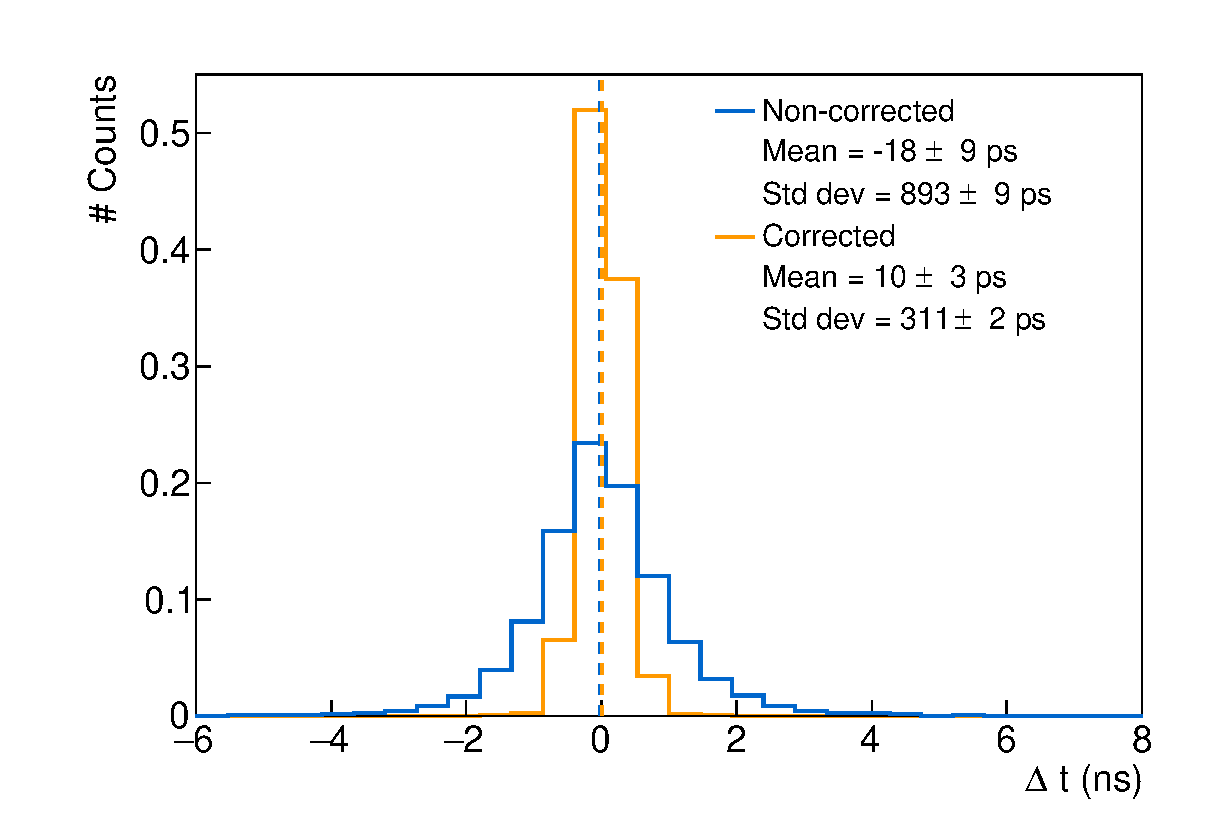
\includegraphics[width=0.7\textwidth]{timedifference/fig_timediff/0nubb_delta_t.eps}
  \captionsetup{justification=justified}
  \caption{$\zeronu$ simulations.
    \label{subfig:0nubb_delta_t}}
\end{subfigure}
\hfill
\begin{subfigure}[t]{1.\textwidth}
  \centering
  \includegraphics[width=0.7\textwidth]{timedifference/fig_timediff/208Tl_delta_t.eps}
  \captionsetup{justification=justified}
  \caption{\Tl\ simulations.
    \label{subfig:208Tl_delta_t}}
\end{subfigure}
\caption{Corrected (orange) and non-corrected (blue) time-of-flight difference between the two electrons.
  (a) $\zeronu$ simulations inside the source foils.
  (b) \Tl\ simulations inside the source foils.
  The first-order selections have been applied.
  The two distributions are normalised.
  $\sigma_{t}=200$~ps and $\sigma_{l}=27.8$~ps.
  \label{fig:delta_t}}
\end{figure}
For $\zeronu$ simulations, the $\Delta t^{corr}$ distribution is centred around zero, as the two electrons are emitted simultaneously inside the source.
Then, the correction on time difference only lowers the standard deviation of the distribution.
For \Tl\ simulations, the mean of the distribution is slightly shifted towards positive values.
Once corrected by the expected times, the mean difference between the two electrons time-of-flights stands at $296~\pm~18$~ps.
This is a direct consequence of the existence of $\beta$+IC delayed events, for which the particle of highest energy is expected to hit a calorimeter block at a time $t^{\text{corr}}_{1}~>~t^{\text{corr}}_{2}$.
The set up calorimeter time uncertainty at $200$~ps allows to be sensitive to this decay as the mean of the distribution is near $294$~ps.
Therefore, a simple way of rejecting the \Tl\ delayed events is to consider the sign of $\Delta t^{\text{corr}}$ and to reject events for which $\Delta t^{\text{corr}}~>~0$.

By applying this selection on $2e$ topologies of $\zeronu$ and \Tl\ simulations for which $E~>~2.7$~MeV, we are able to reject $76$~\% of \Tl\, while selecting $49$~\% of the $\zeronu$ ($\sigma_{t}~=~200$~ps).
The $49$\% of selected signal events is expected as the corresponding $\Delta t^{corr}$ distribution is symmetrical, unlike the one for \Tl\ events.
Although we manage to reject a significant fraction of Thallium events, the impact of this cut is too high on $\zeronu$ events.
Moreover, the uncertainties on time-of-flights are not taken into account in the rejection criterion.
Later in this chapter we consider different levels for this selection and optimise them according to the $\sigma_{t}$ value set up.
%%We study in Sec.~\ref{subsec:selection_optimisation} an optimization of this cut-off, including the influence of the temporal performance of the calorimeter $\sigma_{t}$.

\subsection{Probability cut-off}

At this level it is interesting to consider the internal and exponential probabilities to describe $2e$ topologies and attempt to obtain a higher background rejection.
They seem to be better tools notably because, unlike the $\Delta t^{\text{corr}}$ rejection criterion, they do take into account the time-of-flight uncertainties.
The first one was already used in Chapter~\ref{ch:sensitivity}, and is a widely-used tool to reject non-internal events.
The second was designed specifically for this analysis to identify delayed \Tl\ events, and also depends on the time of flight resolution through the convolution with a Gaussian function.

The idea is this section is to reject \Tl\ events taking into account their two values of internal and exponential probabilities.
Then it is interesting to represent them with a two-dimensional binned histogram of $P_{exp}$ as a function of \Pint, as done is Fig.~\ref{fig:biplot_Pexp_Pint}.
\begin{figure}[!h]
  \centering
  \includegraphics[width=15cm]{timedifference/fig_timediff/PintVSPexp_208Tl_200.eps}
  \caption{Two-dimensional histogram showing the $P_{exp}$ variations as a function of \Pint\ for \Tl\ $2e$ topologies.
    $\sigma_{t}=200$~ps and $\sigma_{l}=27.8$~ps.
    \label{fig:biplot_Pexp_Pint}}
\end{figure}
In this particular example, we picture the variations of \Pint\ and $P_{exp}$ applying ${\sigma_{t}=200}$~ps.
We clearly distinguish three event populations in this histogram.
In order to better understand these variations, we give in Fig.~\ref{fig:proba_cut_ex} three examples of ${(E \otimes G)_{\tau,\mu,\sigma}(\Delta t)}$ distributions, each of them illustrating one of the three zones.
\begin{figure}[!h]
\centering
\begin{subfigure}[t]{0.95\textwidth}
  \centering
  \includegraphics[width=0.64\textwidth]{timedifference/fig_timediff/proba_expo_1.pdf}
  \captionsetup{justification=justified}
  \caption{
    \label{subfig:Proba_cut_1}}
\end{subfigure}
\vskip\baselineskip
\begin{subfigure}[t]{0.95\textwidth}
  \centering
  \includegraphics[width=0.64\textwidth]{timedifference/fig_timediff/proba_expo_2.pdf}
  \captionsetup{justification=justified}
  \caption{
    \label{subfig:Proba_cut_2}}
\end{subfigure}
\vskip\baselineskip
\begin{subfigure}[t]{0.95\textwidth}
  \centering
  \includegraphics[width=0.64\textwidth]{timedifference/fig_timediff/proba_expo_3.pdf}
  \captionsetup{justification=justified}
  \caption{
    \label{subfig:Proba_cut_3}}
\end{subfigure}
\caption{${(E \otimes G)_{\tau,\mu,\sigma}(\Delta t)}$ distributions describing the three areas observed in Fig.~\ref{fig:biplot_Pexp_Pint}.
  (a) $\Delta t^{\text{corr}} \in~]-\infty;0]$.
  (b) $\Delta t^{\text{corr}} \in~]\Delta t_{max};+\infty]$.
  (c) $\Delta t^{\text{corr}} \in~]0;\Delta t_{max}]$.
  \label{fig:proba_cut_ex}}
\end{figure}
\begin{enumerate}
\item \Pint$\in[0;1]$ and $P_{exp}\in[0;0.65]$, with \Pint$>P_{exp}$ (Fig.~\ref{subfig:Proba_cut_1}):\\
  This region corresponds to events for which $\Delta t^{\text{corr}}<0$.
  As the internal $\chi^{2}_{int}$ distribution is symmetrical, such events can have a value of \Pint\ varying from $0$ to $1$.
  Small values of \Pint\ correspond to events with a large negative $\Delta t^{\text{corr}}$ value.
  Conversely, the exponential distribution is not centred in zero.
  Therefore, if we limit to events for which the time difference is negative, we reach an upper bound for the value of the integral ($0.65$ in that case).
  This bound directly depends on the variations of the exponential distribution, therefore on the $\sigma_{t}$ value applied.
\item \Pint$\in[0;0.65]$ and $P_{exp}\in[0;1]$, with $P_{exp}>$\Pint (Fig.~\ref{subfig:Proba_cut_2}):\\
  These events have positive values for $\Delta t^{\text{corr}}$, beyond the ${(E \otimes G)_{\tau,\mu,\sigma}(\Delta t)}$ distribution maximum.
  The smaller the value of \Pint, the lower the probability that both particles were emitted at the same time into the source.
  Besides, for values of $\Delta t^{\text{corr}}$ highly positives, the value of the exponential probability can reach high values, up to $1$.
  The larger the value of $\Delta t^{\text{corr}}$ in positives, the smaller the value of $P_{exp}$.
\item \Pint$\in[0.65;1]$ and $P_{exp}\in[0.65,1]$ (Fig.~\ref{subfig:Proba_cut_3}):\\
  This region is also populated by events for which $\Delta t^{\text{corr}}>0$.
  Unlike the previous case, these events have small $\Delta t^{\text{corr}}$ values, meaning below the maximum of the exponential distribution.
  Also, these events have high internal probability values, as the probability that these two particles were emitted simultaneously is high.
  In the same way as the first bullet, the value of $P_{exp}$ is bounded: the lower bound corresponds to the value of the integral when $\Delta t^{\text{corr}}=0$ (here $0.65$).
  Once again, this bound is deeply related to the value considered for $\sigma_{t}$.
  The exponential probability can be equal to $1$ when $\Delta t^{\text{corr}}$ reaches the maximum of the exponential distribution.
\end{enumerate}

As discussed, the exponential probability quantifies the likelihood that two particles were emitted with a delay corresponding to the radioactive exponential decay with ${\tau=294}$~ps, taking into account the time of flight resolution.
Therefore, we are interested in rejecting events for which values of $P_{exp}$ are high compared with the \Pint\ values.
In that case, a simple selection allowing to discriminate signal $\zeronu$ from delayed \Tl\ event consists in rejecting $2e$ topologies for which $P_{exp}~>~$\Pint\ (this cut-off is pictured in Fig.~\ref{fig:biplot_Pexp_Pint} by a plain black line).
With the previous explanation, we understand that such a cut is strongly linked to the cut on $\Delta t^{\text{corr}}$ presented in the previous sub-section.
%% For $\sigma_{t}=200$~ps, we are able to reject $41$\% of \Tl, while selecting $60$\% of $\zeronu$ $2e$ topologies for which $E>2.7$~MeV.
%% Although we are able to keep more $\zeronu$ events with this probability cut-off than for the one on time-of-flight difference, it is less efficient in rejecting \Tl\ events.

We would like to refine the selection made on the events using the two probabilities.
Regarding the biplot presented in Fig.~\ref{fig:biplot_Pexp_Pint}, the goal is to reject events located in the area $3$ and a part of the events located in area $2$.
Therefore, a more adapted cut-off is to reject events for which ${P_{exp}>0.65}$.
For this selection and ${\sigma_{t}=200}$~ps, we reject $20$\% of \Tl\ and keep $84$\% of $\zeronu$ events.
The proportion of signal events kept with this selection is satisfying.
Nevertheless the efficiency of \Tl\ rejection is almost $4$ times lower than for the time-of-flight selection presented in Sec.~\ref{subsec:tof_cutoff}.



\subsection{Influence of the calorimeter time resolution}
\label{subsec:calo_sigma}

We study in this subsection the influence of the calorimeter timing resolution on event selections, using the cut-offs presented above.
We consider values for $\sigma_{t}$ in the [$0$ - $400$]~ps range.

In Sec.~\ref{subsec:tof_cutoff} we presented rejection efficiencies for a ${\Delta t^{corr}>0}$~ps selection, with ${\sigma_{t}=200}$~ps.
In Fig.~\ref{fig:eff_cut_delta_t_sigma} is presented the $\zeronu$ selection efficiency with the rejection efficiency of \Tl, for values of $\sigma_{t}$ running from the ideal $0$~ps, to $400$~ps.
\begin{figure}[!h]
  \centering
  \includegraphics[width=13cm]{timedifference/fig_timediff/compare_sigma_cut_delta_t.pdf}
  \caption{$\zeronu$ selection efficiency as a function of \Tl\ rejection.
    Each curve corresponds to a given value of $\sigma_{t}$ from $0$ to $400$~ps.
    Each data point corresponds to a minimum value for $\Delta t^{corr}$ applied on selected $2$ topologies from $0$ to $650$~ps.
    the optimised value of $\sigma_{l}=27.8$~ps is applied.
    \label{fig:eff_cut_delta_t_sigma}}
\end{figure}
Each point corresponds to a $\Delta t^{corr}$ level applied on the selected $2e$ topologies, from ${\Delta t^{corr}>0}$ to ${\Delta t^{corr}>650}$~ps.
For ${\Delta t^{corr}>0}$ and $\sigma_{t}=200$~ps, we get back to the result given previously.
Nevertheless, for this time uncertainty, an optimised value for the $\Delta t^{corr}$ cut level, called \emph{maximum efficiency point}, is found at ${\Delta t^{corr}>250}$~ps as it optimises the signal selection and \Tl\ background rejection efficiencies.
Such a point can be found for each of the five $\sigma_{t}$ values presented.
The more precisely the time-of-flight is measured in the calorimeter, the better this point is determined.
Indeed, the worse this resolution is, the more linear the distribution tends to be, and therefore the more difficult it is to discriminate delayed events from those emitted simultaneously such as those of $\zeronu$.
Especially, for an ideal calorimeter where the timing measurement would be perfect, we could reach $80$\% of \Tl\ rejection, while keeping $90$\% of signal events.

As discussed, the variations of \Pint\ and $P_{exp}$ are bound to the value of $\sigma_{t}$, thus the levels applied on \Pint\ and $P_{exp}$ must be adapted to match these variations.
Eight \Pint$/P_{exp}$ biplots are given in Fig.~\ref{fig:biplot_Pexp_Pint_sigma}, for $\sigma_{t}=0$, $100$, $300$ and $400$~ps both for $\zeronu$ and \Tl\ $2e$ selected topologies (the ${\sigma_{t}=200}$~ps case is already given in Fig.~\ref{fig:biplot_Pexp_Pint}).
%%\begin{changemargin}{-10cm}{10cm}
\begin{figure}[!h]
\centering
\begin{subfigure}[t]{0.49\textwidth}
  \centering
  \includegraphics[width=0.76\textwidth]{timedifference/fig_timediff/PintVSPexp_208Tl_0.eps}
  \captionsetup{justification=justified}
  \caption{\Tl simulations, ${\sigma_{t}=0}$~ps.
    \label{subfig:}}
\end{subfigure}
\hfill
\begin{subfigure}[t]{0.49\textwidth}
  \centering
  \includegraphics[width=0.76\textwidth]{timedifference/fig_timediff/PintVSPexp_0nubb_0.eps}
  \captionsetup{justification=justified}
  \caption{$\zeronu$ simulations, ${\sigma_{t}=0}$~ps.
    \label{subfig:}}
\end{subfigure}
%%\vskip\baselineskip
\begin{subfigure}[t]{0.49\textwidth}
  \centering
  \includegraphics[width=0.76\textwidth]{timedifference/fig_timediff/PintVSPexp_208Tl_100.eps}
  \captionsetup{justification=justified}
  \caption{\Tl simulations, ${\sigma_{t}=100}$~ps.
    \label{subfig:}}
\end{subfigure}
\hfill
\begin{subfigure}[t]{0.49\textwidth}
  \centering
  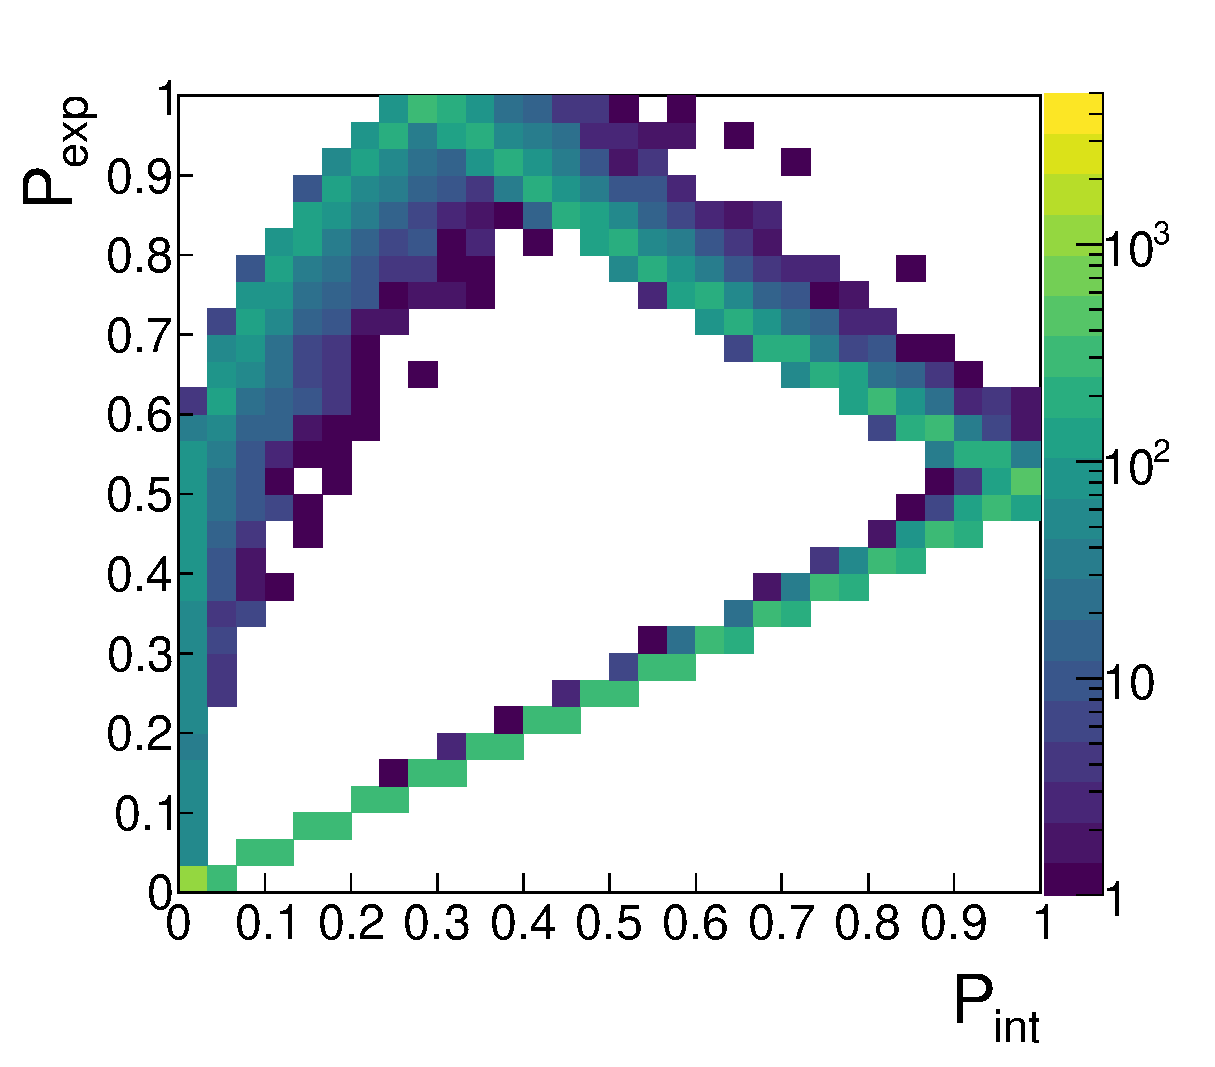
\includegraphics[width=0.76\textwidth]{timedifference/fig_timediff/PintVSPexp_0nubb_100.eps}
  \captionsetup{justification=justified}
  \caption{$\zeronu$ simulations, ${\sigma_{t}=100}$~ps.
    \label{subfig:}}
\end{subfigure}
%%\vskip\baselineskip
\begin{subfigure}[t]{0.49\textwidth}
  \centering
  \includegraphics[width=0.76\textwidth]{timedifference/fig_timediff/PintVSPexp_208Tl_300.eps}
  \captionsetup{justification=justified}
  \caption{\Tl simulations, ${\sigma_{t}=300}$~ps.
    \label{subfig:}}
\end{subfigure}
\hfill
\begin{subfigure}[t]{0.49\textwidth}
  \centering
  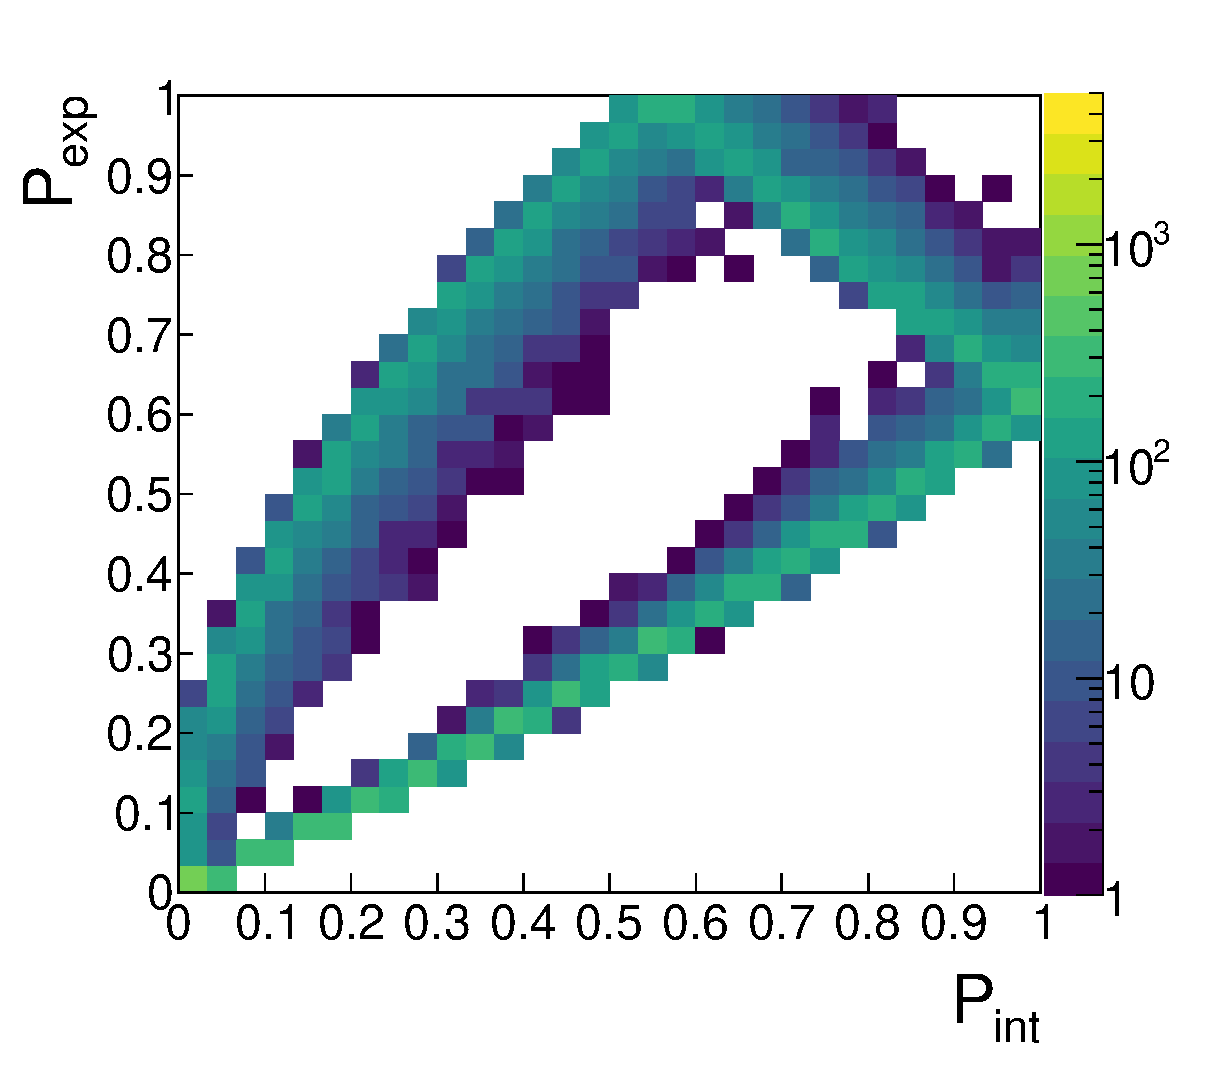
\includegraphics[width=0.76\textwidth]{timedifference/fig_timediff/PintVSPexp_0nubb_300.eps}
  \captionsetup{justification=justified}
  \caption{$\zeronu$ simulations, ${\sigma_{t}=300}$~ps.
    \label{subfig:}}
\end{subfigure}
%%\vskip\baselineskip
\begin{subfigure}[t]{0.49\textwidth}
  \centering
  \includegraphics[width=0.76\textwidth]{timedifference/fig_timediff/PintVSPexp_208Tl_400.eps}
  \captionsetup{justification=justified}
  \caption{\Tl simulations, ${\sigma_{t}=400}$~ps.
    \label{subfig:}}
\end{subfigure}
\hfill
\begin{subfigure}[t]{0.49\textwidth}
  \centering
  \includegraphics[width=0.76\textwidth]{timedifference/fig_timediff/PintVSPexp_0nubb_400.eps}
  \captionsetup{justification=justified}
  \caption{$\zeronu$ simulations, ${\sigma_{t}=400}$~ps.
    \label{subfig:}}
\end{subfigure}
\caption{\Pint$/P_{exp}$ biplots for different $\sigma_{t}$ values for \Tl\ and $\zeronu$ simulations.
  \label{fig:biplot_Pexp_Pint_sigma}}
\end{figure}
%%\end{changemargin}
Depending on $\sigma_{t}$, the area to be rejected moves towards higher values of \Pint.
Taking this into consideration, optimised values for \Pint\ have been set up, summarised in Tab.~\ref{tab:Pint_cutoff_sigma}.
\begin{table}[!h]
  \centering
  \begin{tabular}{|c|c|c|c|c|c|}
    \hline
    $\sigma_{t}$ (ps) & $0$ & $100$ & $200$ & $300$ & $400$ \\
    \hline\hline
    \Pint\ cut-off & [$0.05$ - $0.3$] & [0.25 - 0.6] & [0.4 - 0.7] & [0.5 - 0.8] & [0.55 - 0.85] \\
    \hline
  \end{tabular}
  \caption{Range of \Pint\ for which events are rejected.
    An additional cut-off with \Pint$<0.01$ and $P_{exp}<0.01$ is also applied.
    \label{tab:Pint_cutoff_sigma}}
\end{table}
To find an optimal value of $P_{exp}$ to be applied, several cut-offs are set up from $P_{exp}>0$ to $0.95$, and associated with the \Pint\ cut-offs presented in the previous table, in order to reject the required area.
Following the work done for the $\Delta t^{corr}$ cut-off, results are presented in Fig.~\ref{fig:eff_cut_proba_sigma} on an efficiency selection diagram.
\begin{figure}[!h]
  \centering
  \includegraphics[width=13cm]{timedifference/fig_timediff/compare_sigma_cut_proba.pdf}
  \caption{$\zeronu$ selection efficiency as a function of \Tl\ rejection.
    Each point corresponds to a minimal $P_{exp}$ value applied on the selected $2e$ topologies.
    \Pint\ selections are also applied, their value depending on the $\sigma_{t}$ value (Tab.~\ref{tab:Pint_cutoff_sigma}).
    $\sigma_{l}=27.8$~ps.
    \label{fig:eff_cut_proba_sigma}}
\end{figure}
The calorimeter timing measurement has a great influence, especially on \Tl\ events rejection.
Evolution of selection efficiencies for ${\sigma_{t}<200}$~ps are very similar, reaching a plateau for ${\sim P_{exp}>0.25}$ allowing to reject $20$\% of \Tl\ while keeping $85$\% of $\zeronu$.
Below $\sigma=100$~ps the background rejection is improved despite a loss in signal selection efficiency, up to reaching $\sim45$\% of \Tl\ rejection and $\sim80$\% signal selection for an ideal calorimeter.
The plateau is reached at $P_{exp}>0.2$ for $\sigma_{t}=100$~ps and $P_{exp}>0.15$ for $\sigma_{t}=0$~ps.

A better Thallium rejection can be obtained with the simple selection on time-of-flights, but the probability one has the main advantage to be more accurate as it takes into account the calorimeter time measurement uncertainties.
Moreover, even if variations of selection/rejection of this diagram are not as pronounced as for the $\Delta t^{corr}$ cut-off, a strong assumption can be made: the more we are precise on time-of-flight measurements, the more we are able to reject \Tl\ events while keeping a satisfying part of signal.
During the calorimeter R\&D, a great effort has been made to improve the optical modules energy resolution compared to NEMO-$3$, notably because it allows to have a better background rejection, and thus to decrease its contribution to the $\zeronu$ search.
Finally, in view of these results, a good timing precision in calorimeter blocks is also important when it concerns background rejection, and especially the identification of $\beta$+IC delayed \Tl\ decays.
Nevertheless, to give a final conclusion on the usefulness of the $\Delta t^{corr}$ and probability cut-offs, one have to study its impact on the final sensitivity of the detector, which is dealt with in the next section.

%% \begin{figure}[!h]
%%   \centering
%%   \includegraphics[width=13cm]{timedifference/fig_timediff/efficiency_proba.pdf}
%%   \caption{$\zeronu$ selection efficiency as a function of \Tl\ rejection.
%%     Each data point corresponds to a given value of $\sigma_{t}$, decrementing in $50$~ps steps.
%%     First order selections applied on $\zeronu$ and \Tl\ simulations.
%%     $\sigma_{l}=27.8$~ps.
%%     \label{fig:eff_proba_sigma}}
%% \end{figure}


\section{Impact of \Tl\ rejection on the experiment's sensitivity}
\label{sec:Tl_sensitivity}

In the previous sub-section were presented results for $\Delta t^{corr}$ and optimised probability cut-offs, and the influence of the calorimeter time resolution on these rejection techniques was reviewed.
Nevertheless, to properly quantify the effectiveness of these cut-off, one have to study their impact on the final detector sensitivity ($500$~kg.y exposure).
To do so, the procedure described in Chapter~\ref{ch:sensitivity} is applied to the $2e$ topologies selected (after the application of $\Delta t^{corr}$ or probability cut-offs), for signal and backgrounds considered ($\twonu$, \Bi, \Tl\ and \Rn).

\subsection{Sensitivity results}

The variations of the sensitivity are presented in Fig.~\ref{fig:T12_cut} for three values of $\sigma_{t}$ at $1$~MeV, as a function of the cut-off levels applied.
\begin{figure}[!h]
\centering
\begin{subfigure}[t]{1\textwidth}
  \centering
  \includegraphics[width=0.98\textwidth]{timedifference/fig_timediff/compare_sigma_cut_delta_t_T12.pdf}
  \captionsetup{justification=justified}
  \caption{$\Delta t^{corr}$ cut-off.
    \label{subfig:T12_cut_deltat}}
\end{subfigure}
\begin{subfigure}[t]{1\textwidth}
  \centering
  \includegraphics[width=0.98\textwidth]{timedifference/fig_timediff/compare_sigma_cut_proba_T12.pdf}
  \captionsetup{justification=justified}
  \caption{Probability cut-off.
    \label{subfig:T12_cut_proba}}
\end{subfigure}
\caption{(Top pad) $\Tbeta$ at $90$\% CL and (bottom pad) optimised ROI, as a function of the minimal value of $\Delta t$ applied on the selected $2e$ topologies.
    Results are given for $\sigma_{t}=0$, $200$ and $400$~ps at $1$~MeV, and $\sigma_{l}=27.8$~ps.
  \label{fig:T12_cut}}
\end{figure}
For these two figures, the more the $x$-values increase, the more the applied cut is released.
In both cases sensitivity results converge towards $\sim2.4\times10^{25}$~years, for very loose values of the selection.
%% This value is slightly different than the final results given in Chapter~\ref{ch:sensitivity}, due to the energy cut-off which is firstly applied on $2e$ topologies in the current study (Sec.~\ref{subsec:energy_seletion}).

Regarding the influence of $\Delta t^{corr}$ selection, a sensitivity improvement can eventually be obtained by applying this selection, depending on the value of $\sigma_{t}$ considered for the calorimeter (Fig.~\ref{subfig:T12_cut_deltat}).
\begin{itemize}
\item $\sigma_{t}=0$~ps at $1$~MeV: an improvement of $12$\% on the sensitivity is observed for events rejected if $\Delta t^{corr}>200$~ps.
  This is consistent with the \Pb\ metastable level of $294$~ps to which we are very sensitive with such ideal value of the calorimeter resolution.
\item $\sigma_{t}=200$~ps at $1$~MeV: a slighter improvement of $6$\% is reached for $\Delta t^{corr}>550$~ps.
  As the calorimeter time resolution is reduced, compared with the first ideal case, a smaller improvement can be obtained, for a loose value of the applied cut.
\item $\sigma_{t}=400$~ps at $1$~MeV: the resolution is too degraded for an improvement to be obtained with such a time-of-flight cut-off.
\end{itemize}

Concerning the influence of probability selection, values of $\Tbeta$ also converge towards a unique value, attained for $P_{exp}>1$, meaning all the events are selected for such a level.
In other words, the more restrictive this cut is, the more the sensitivity is reduced.
The least unfavourable case is obtained for the ideal calorimeter resolution case, with stagnation of the values on a plateau, for most of the applied cut-off levels.
Even if it is less wide, a plateau is also reached for $\sigma_{t}=200$~ps.


\subsection{Expected number of background}

The influence of the $\Delta t^{corr}$ selection on the number of expected background events in the optimised ROI is presented in Tab.~\ref{tab:Nbkg_deltat_cut}.
\begin{table}[h!]
  \centering
  \begin{tabular}{|c|c|c|c|}
    \hline
    $\sigma_{t}$ (ps) & $0$ & $200$ & $400$ \\
    ROI (MeV) & [$2.7$;$2.95$] & [$2.7$;$2.9$] & [$2.7$;$2.95$] \\
    Minimal $\Delta t^{corr}$ (ps) & $200$ & $550$ & $650$ \\
    $\Tbeta$ ($90$\% CL) ($\times10^{25}$~y) & $2.7$ & $2.5$ & $2.4$ \\
    $\mbb$ ($90$\% CL) (eV) & $[0.11-0.22]$ & $[0.11-0.22]$ & $[0.12-0.23]$ \\
    \hline\hline
    $\epsilon_{0\nu}$ & $14.6$\% & $14.2$\% & $12.9$\% \\
    \hdashline
    $\twonu$  & $10.8$ & $10.8$ & $9.58$ \\
    \Tl  & $9.52$ & $13.3$ & $13.4$ \\
    \Bi  & $42.9$ & $42.0$ & $39.2$ \\
    \Rn  & $1.12$ & $1.12$ & $1.04$ \\
    Total & $64.4$ & $67.2$ & $63.2$ \\
    \hline
  \end{tabular}
  \caption{Expected number of background events in the optimised ROI, for the exposure of the SuperNEMO final detector ($500$~kg.y).
    Three values of $\sigma_{t}$ are considered for which the best $\Delta t^{corr}$ is applied.
    \label{tab:Nbkg_deltat_cut}}
\end{table}
Three values of $\sigma_{t}$ are considered, and for each of them the best level for this cut, determined in the previous sub-section, is applied.
The best rejection of Thallium is reached for the ideal calorimeter time resolution, as the two electrons time-of-flights are measured precisely.
For $\sigma_{t}=200$~ps, a smaller amount of Thallium background is rejected, but the $\zeronu$ selection efficiency remains stable.
This selection efficiency is affected when the time resolution is degraded to $\sigma_{t}$, thus when the delayed events are badly discriminated compared with the simultaneous ones.
As expected, other background events ($\twonu$, \Bi\ and \Rn) are not significantly affected by this selection.

As discussed, the probability cut-offs applied on $2e$ topologies only degrade the final sensitivity to the $\zeronu$ process.
To quantify its impact on the background rejection, we present in Tab.~\ref{tab:Nbkg_proba_cut} the expected number of background in the optimised ROI, for two different levels for the $P_{exp}$ selection, one at $0.5$ and the other one very loose.
\begin{table}[h!]
  \centering
  \begin{tabular}{|c|c|c|}
    \hline
    ROI (MeV) & [$2.7$;$2.9$] & [$2.7$;$2.9$] \\
    Minimal $P_{exp}$ & $0.5$ & $0.95$ \\
    $\Tbeta$ ($90$\% CL) ($\times10^{25}$~y) & $2.2$ & $2.4$ \\
    $\mbb$ ($90$\% CL) (eV) & $[0.12-0.24]$ & $[0.12-0.23]$ \\
    \hline\hline
    $\epsilon_{0\nu}$ & $12.1$\% & $13.9$\% \\
    \hdashline
    $\twonu$  & $9.83$ & $10.8$ \\
    \Tl  & $16.3$ & $21.0$ \\
    \Bi  & $38.4$ & $42.0$ \\
    \Rn  & $0.596$ & $0.596$ \\
    Total & $65.1$ & $74.4$ \\
    \hline
  \end{tabular}
  \caption{Expected number of background events in the optimised ROI, for the exposure of the SuperNEMO final detector ($500$~kg.y).
    The time resolution is taken as $\sigma_{t}=200$~ps.
    Two levels of $P_{exp}$ cut are compared, $0.5$ and $0.95$.
    \label{tab:Nbkg_proba_cut}}
\end{table}
Even if it affect the $\zeronu$ selection efficiency, this selection allows to reject $5$ events of \Tl\ inside the ROI for the SuperNEMO final detector.

These two selections were implemented in order to reject \Tl\ events and they have fulfilled this role.
The $\Delta t^{corr}$ selection allowed to improve the sensitivity by $12$\% for a perfect calorimeter time resolution.
Finally, the final detector sensitivity is greatly affected by this timing measurement precision.



\section{Conclusion}

During this chapter we have defined or specified analysis tools adapted to the rejection of background.
In particular, a so-called exponential probability law has been defined to describe the internal events of delayed Thallium.
Although the cut-off based on the electron time-of-flight is very satisfactory for rejecting this last background, the associated cut-off in internal and exponential probability makes it possible to be more precise since it takes into account the errors made on the time-of-flight measurements in the calorimeter.
These rejection could be tested on site using a $^{232}$U calibration source, a parent of \Tl\ nucleus, inside the calorimeter to check the \Tl\ rejection using time-of-flight.

We have determined the influence the time resolution has on the various defined cut-off efficiencies.
The worse this resolution is, the more difficult it is to discriminate thallium events from signal events.
Improving the time resolution of the calorimeter was not a direct purpose of the R\&D programme, however it has benefited from the high light output achieved to meet the energy resolution goals.
The time resolution of the optical modules has been monitored at every stage of the R\&D programme but remains to be precisely determined.
This is precisely the purpose of the next chapter, which describes how we determined the time resolution of the optical modules of the demonstrator calorimeter with a \Co\ source.

%% \chapter{Characterisation of the calorimeter resolution}

Optical modules have been characterised before installation.
Most of the \Co\ $\beta$ desintegrations are followed by the emission of two $\gamma$s in coincidence (see Fig.~\ref{fig:Co_decay_scheme}).
The idea is to use this source to calibrate in time optical modules of SuperNEMO demonstrator by placing it behind the main calorimeter walls (the demonstrator being closed since ...) and using the two coincidence $\gamma$s.
Performing simulations of \Co\ desintegrations



\section{Calibration with a Cobalt source}
\subsection{Experimental setting and goal}
\subsection{Data taking at LSM}
\subsection{Analysis}
\subsection{Results}

\begin{figure}
  \centering
  \includegraphics[width=10cm]{CoSource/fig_CoSource/Co_decay_scheme.png}
  \label{fig:Co_decay_scheme}
  \caption{Decay scheme of Cobalt $60$.
  After the $\beta$ desintegration $99.88$\%, }
\end{figure}

%% \include{efficiency/efficiency}
\chapter{Detector commissioning}
\label{ch:commissioning}

The commissioning of the SuperNEMO demonstrator has begun in $2019$ and first calorimeter data was taken.\\
The calorimeter of SuperNEMO is segmented in $712$ optical modules (OM), each composed by a coupling between a photomultiplier tube (PMT) and a polystyrene scintillator bloc (see Sec.~\ref{sec:calorimeter} for more details).
The divider of a PMT is connected to $2$ cables, one providing the high voltage (HV), the other one, called signal cable, is a coaxial cable collecting and transporting the charge provided by the PMT.\\
By the summer $2020$, the SuperNEMO demonstrator will be encapsulated in an anti radon tent.
The so called \emph{patch panel} will insure passage of cables from the inside, to the outside of the anti radon tent, therefore doubling the amount of cables needed for the calorimeter.
We refer to the cables running from detector to patch panel as \emph{internal} cables, and the cables from patch panel to the electronic boards as \emph{external} cables.
Consequently, regarding only the calorimeter part, 2848 cables were cut, assembled, connector-mounted, transported and installed at LSM.
Then the check of every cable condition is mandatory to control and eventually fix them.

\section{Reflectometry analysis}
\label{sec:reflecto}

\subsection{Goal of the reflectometry analysis}

Taking into account the final demonstrator design, each coaxial length was determined, cables were cut and labelled in LAL, Orsay.
All external coaxial cables were designed to be $7$ meters-long -- the distance between electronic boards and patch panel being the same for all channels at electronic boards -- and internal cable lengths have been adapted to fit the distance from the patch panel to each optical module.
Then, cutting and labelling all cables lasted several weeks.
After all cables were transported and installed at LSM, we had to check each coaxial cable condition, for several reasons:
\begin{itemize*}
\item check if no cable was damaged during the transport and the installation;
\item control if no swap between cables has been made during cable labelling or calorimeter cabling,
\item check if the coaxial cable was cut at the right length,
\item more importantly estimate the signal time delay due to the cable lengths: knowing that the velocity of electrons in the coaxial cables has a known constant value, the longer is the cable, the more the signal takes time to travel from the PMT to the electronic channel.
  Therefore, each coaxial cable length has to be characterised, especially if we want to do time coincidences between two signals in two different channels.
\end{itemize*}
To do so, a pulse, called \emph{primary} pulse, is generated at the electronic board readout.
The signal will travel all along the coaxial cable, from the electronic board to the PMT divider.
Whether the cable is correctly connected to the PMT or not, the signal reflects at the other end.
\begin{figure}[h]
  \centering
  \begin{subfigure}[b]{0.3\textwidth}
    \centering
    \includegraphics[width=1.1\textwidth]{commissioning/fig_commissioning/scheme_reflecto.pdf}
    \captionsetup{justification=centering}
    \caption{Normal reflection at PMT divider.
      \label{subfig:reflecto_normal}}

  \end{subfigure}
  \hfill
  \begin{subfigure}[b]{0.3\textwidth}
    \centering
    \includegraphics[width=1.1\textwidth]{commissioning/fig_commissioning/scheme_reflecto_1.pdf}
    \captionsetup{justification=centering}
    \caption{Cable not connected at PMT.
      \label{subfig:reflecto_pmt}}

  \end{subfigure}
  \hfill
  \begin{subfigure}[b]{0.3\textwidth}
    \centering
    \includegraphics[width=1.1\textwidth]{commissioning/fig_commissioning/scheme_reflecto_2.pdf}
    \captionsetup{justification=centering}
    \caption{Cable not connected at patch panel.
      \label{subfig:reflecto_pp}}

  \end{subfigure}
  \caption{A representation of pulses sent in a cable for the reflectometry analysis is given.
    The electronic boards are symbolised by the black chip, and the patch panel by the red vertical bar.
    Three scenario where a primary pulse is sent in one cable (represented in grey), are represented.
    (a) The cable is well connected at the patch panel and at the PMT. The signal reflects at the PMT divider.
    (b) The cable is not connected at PMT and the signal is reflected at the end of the cable.
    (c) The cable is not connected at patch panel and the signal is reflected at the end of the external cable.\label{fig:reflecto_scheme}}

\end{figure}
Then the signal travels back from the PMT to the electronic board channel, where it is recorded by the acquisition.
We called this recorded reflected pulse \emph{secondary} pulse.
An example of the total recorded signal is displayed in Fig.~\ref{subfig:total_waveform}.
In order to accumulate enough statistics, we send thousands of pulses in each coaxial cable.
The analyses of the shape and of the arrival time of those secondary pulses for each channel is called \emph{reflectometry}, and allow us to check the coaxial cable conditions and to control their lengths.

\subsection{Pulse timing: controlling cable lengths}
\label{subsec:timing}

The first step of this analysis is to experimentally determine the length $l_{j}^{m}$ for all signal cables $j$ installed on the demonstrator.
This length is defined as
\begin{equation}
  l_{j}^{m}= 0.5\,t_{j}\,v_{p}\, ,
\end{equation}
where $t_{j}$ stands as the time made by the electrons to do a round trip between one electronic channel and one PMT, and $v_{p}$ is the velocity of electrons in the coaxial cables, which can be expressed as a fraction of light speed in vacuum, $c$.
The time difference $t_{j}$ between the primary pulse and the secondary pulse is written as
\begin{equation}
  t_{j} = \braket{t_{\text{secondary pulse}}-t_{\text{primary pulse}}}_{p} \, \text{,}
\end{equation}
$\braket{}_{p}$ being the average over all pulses sent in one single cable $j$.
The velocity $v_{p}$ is supplied by the cable manufacturer as
\begin{equation*}
  v_{p}=\frac{c}{\sqrt{\epsilon_{r}}}\,\text{,}
\end{equation*}
with $\epsilon_{r}$ the relative dielectric constant of the material.
Therefore, this celerity depends on the components.
For the coaxial cables chosen in the demonstrator design, the data sheet of the cable gives ${v_{p}=0.69\,c}$.
A study is performed to verify experimentally the value of $v_{p}$.
Three cables of different lengths are measured with a precision of $1$ cm.
A thousand of primary pulses are sent in each of the three cables, then the time for each secondary pulse is recorded.
At the end, we have three independent measures of the velocity $v_{p}$ in the used coaxial cables.
On Fig.~\ref{fig:celerity} is displayed the lengths $l_{j}$ as a function of the times $t_{j}$.
\begin{figure}[h]
  \centering
  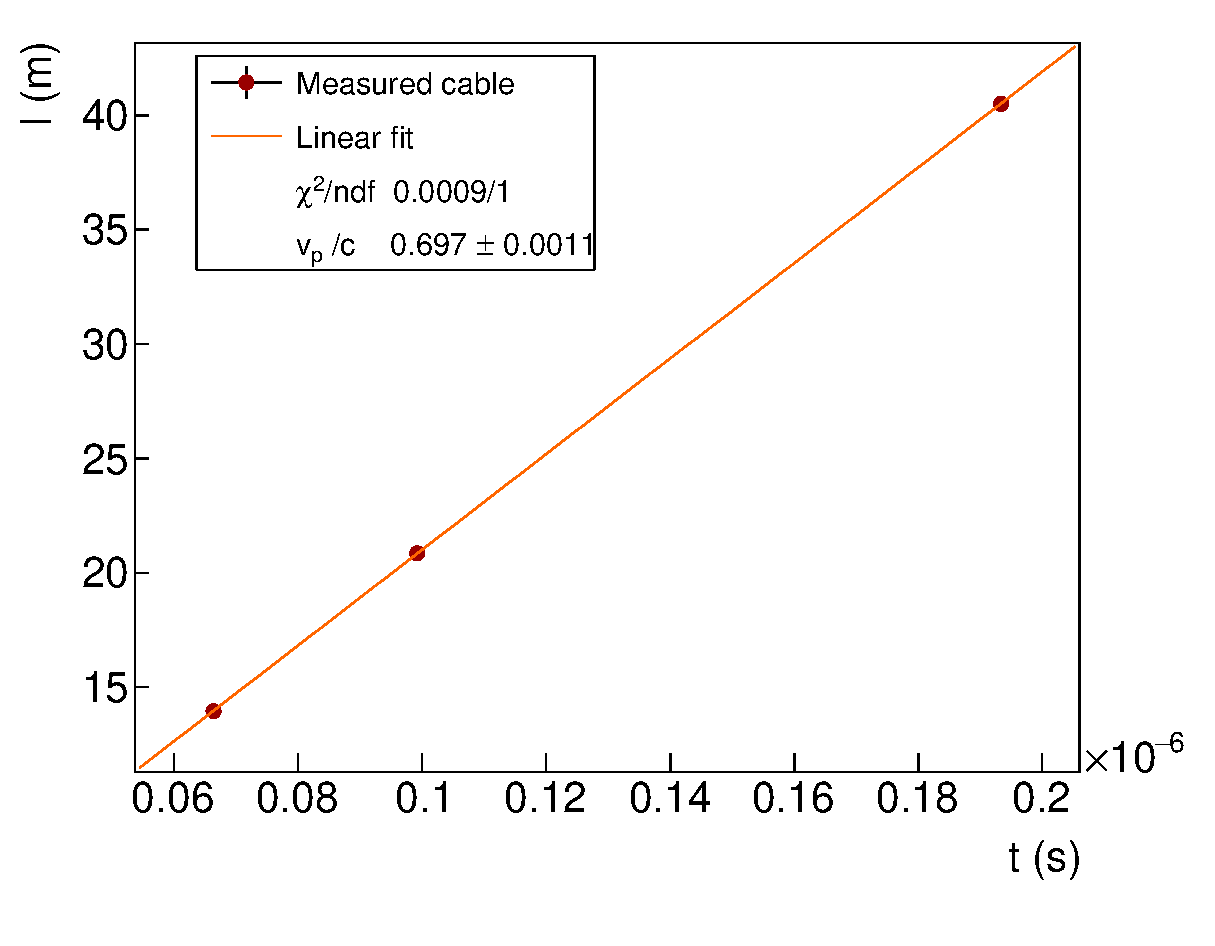
\includegraphics[width=15cm]{commissioning/fig_commissioning/celerity.eps}
  \caption{Three different lengths $l_{j}$ of cables are measured.
    Pulses are sent inside all cables.
    The lengths $l_{j}$ are plotted as a function of the time differences $t_{j}$ between primary and secondary pulses.
    The value of $v_{p}/c$ fitted from the data points is displayed.
    This value of $0.697\pm 0.0011$ shows the compatibility with the one supplied by the constructor, of $0.69$ c.
    \label{fig:celerity}}
\end{figure}
The fitted value of $v_{p}/c = 0.697\pm 0.0011$ is displayed and shows a compatibility up to $7\sigma$ with the data sheet.

As we want to determine the time interval $t_{j}$, we have to define what is the \emph{time} of a pulse.
In this analysis, we use a technique called Constant Fraction Discriminator (CFD), providing an amplitude-independent information about time of a pulse.
This algorithm aims at tracking a signal and defining its time arrival at a given fraction $f$ of its maximal amplitude.
The two main advantages of this technique is that it provides an efficient rejection of the noise in the acquisition window, and gives a good resolution on the measured time.
Nevertheless, the possible influence of the chosen value for the $f$ parameter on this time resolution has to be investigated.
We perform such a study in Sec.~\ref{subsec:CFD}.
We concluded that the highest precision on the time measurement arises for $f = 40\%$, and we adopt this value for the following analysis.
A graphic representation of the CFD time search is given in fig.~\ref{subfig:zoom_secondary}.
\begin{figure}[h]
\centering
\begin{subfigure}[t]{0.7\textwidth}
  \centering
  \includegraphics[trim={1.2cm 3.5cm 1.7cm 3.1cm},clip,width=1\textwidth]{commissioning/fig_commissioning/CFD_example.pdf}
  \captionsetup{justification=centering}
  \caption{Total recorded waveform
    \label{subfig:total_waveform}}
\end{subfigure}
\hfill
\begin{subfigure}[t]{0.7\textwidth}
  \centering
  \includegraphics[trim={1.2cm 1.5cm 1.7cm 3.1cm},clip,width=1\textwidth]{commissioning/fig_commissioning/CFD_example_zoom.pdf}
  \captionsetup{justification=centering}
  \caption{Zoom on secondary pulse
    \label{subfig:zoom_secondary}}
\end{subfigure}
\caption{(a) Total recorded waveform: primary pulse (left) and secondary the pulse (right).
  (b) Zoom on the secondary pulse.
    A representation of time computed with a Constant Fraction Discriminator (CFD) is provided.
    Its maximal amplitude (red dotted line) and its fraction for $\text{f}=40\%$ (green dotted line) are displayed.
    The time $\text{T}_{\text{pulse}}$ (orange dotted line) represents the time of arrival of the secondary pulse computed with CFD, with the fraction $\text{f}=40\%$.
  \label{fig:CFD}}
\end{figure}
As we want to measure the installed cable lengths $l^{m}_{j}$, and compare them to the initially designed ones, $l^{d}_{j}$, we define the length difference $\Delta L_{j}$ as:
\begin{equation}
  \Delta L_{j} = l^{m}_{j}-l^{d}_{j}\, .
\end{equation}
On Fig.~\ref{fig:LengthDiff} is displayed the distribution $\Delta L$ for all the measured lengths.
\begin{figure}[h]
  \centering
  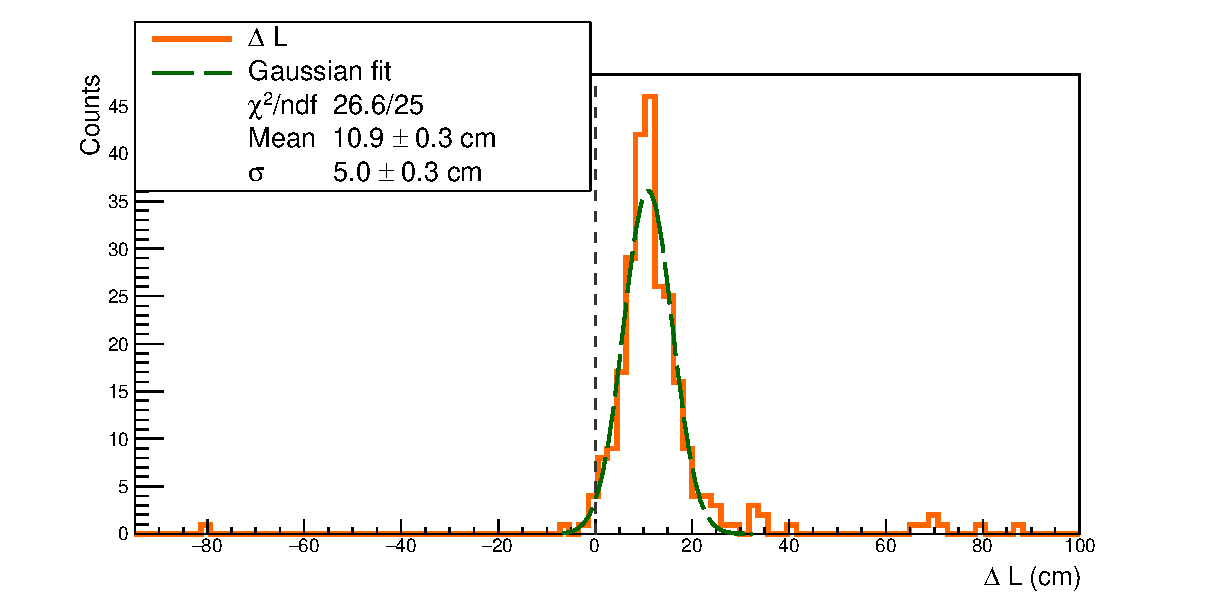
\includegraphics[width=15cm]{commissioning/fig_commissioning/length_diff.eps}

  \caption{The distribution of difference between the measured lengths $l^{m}$ and the expected lengths $l^{d}$ is displayed in orange solid line.
    The black dashed line represents the case where $l^{m}_{j} = l^{d}_{j} \;\forall j$.
    The Gaussian fit (green dashed line) presents a mean of $10.9 \pm 0.3$ cm.
    Some data points considered as outliers are beyond $3\sigma$.
    \label{fig:LengthDiff}}
\end{figure}
In hypothetical perfect conditions, all the cables should fit the design length, in other words, $l^{d}_{j} = l^{m}_{j}$.
Consequently the $\Delta L$ distribution should a peak at zero, as materialised by the black dashed line.
However, in real conditions, the measured length can be different from the designed one, leading the $\Delta L$ distribution plotted in orange solid line.
We conclude that the observed cable length $l^{m}$ differs from $l^{d}$ by $+10.9\pm 0.3$ cm, meaning that cables are longer than expected in average.
This may reveal a bias coming from the device used to cut the cables.
In fact, during cable cutting work, we noticed that the cutting device had a tendency to slip, probably leading to cables with extra lengths.
We assumed the cutting device has a given probability to slip for one meter of cable.
If this is the case, the probability for the device to give extra length should increase with the cable length.

To verify this assumption, we plot on Fig.~\ref{fig:CutBias} the length difference $\Delta L$ as a function of the initial design length $l^{d}$ (cyan).
From those data points, we compute a linear fit (orange solid line), parameterised as $y = \alpha x + \beta$, revealing that the cutting device presents two different biases.
\begin{figure}[h]
  \centering
  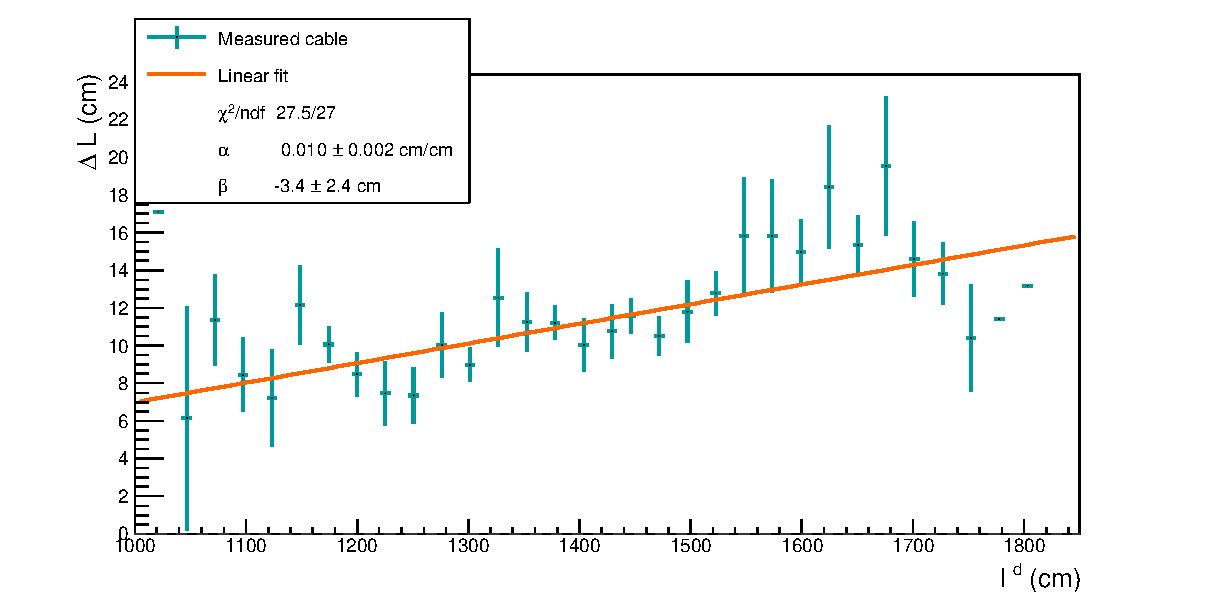
\includegraphics[width=15cm]{commissioning/fig_commissioning/cut_biais.eps}

  \caption{$\Delta L$ is plotted with $l^{d}$ (cyan), where $l^{d}$ is averaged for all the lengths designed to have the same value, being at the origin of vertical error bars.
    In black dashed line is represented the case where $l^{m} = l^{m}$.
    Data points are fitted by $\alpha x + \beta$, with $\alpha > 0$ and $\beta < 0$, revealing the two biases of the cutting device.
    \label{fig:CutBias}}
\end{figure}
The value of $\beta$ shows that the cutting device systematically took away $3.4$ cm of each cable.
Nevertheless, as the shortest cable was designed to be 10 meters long, there are no important consequences of this bias on the length difference $\Delta L$.
Besides, the slope $\alpha = 0.010\pm 0.002$ of the linear fit reveals that the cutting device adds one centimetre for every meter of cable, being compatible with the hypothesis on the cutting device sliding.
Hopefully this bias is not problematic as it makes most of the actual cable lengths longer than the design, while shorter lengths could have lead to systematic connection issues to PMTs.
However, we notice that a few cables have been cut too short by mistake, the worse of them being $80$ centimetres shorter than expected.
Fortunately, this cable  was successfully connected to PMT despite this deficit.
On the contrary, few cables have a large extra length.
This probably is due to human punctual mistakes on top of the observed bias, but without any strong consequences for the calorimeter operation.
In conclusion, no important mistakes have been made when cutting cables, and we had no issue for connecting the only problematic cable.

If the main goal of this study is to check the lengths of coaxial cables, it also aims at correcting the time of recorded events, from the time made by the signal to travel from a PMT to an electronic channel.
taking into account the time for the signal to travel through cables.
This become possible with the reflectometry study we performed.
Knowing real lengths of cables and using the celerity of the signal, we deduce the time needed for the signal to travel from one given PMT divider to the electronic boards.
Then we can correct event times.

As explained previously, the time $t_{j}$ gives information about the length of the cable $j$.
We remind the coaxial cables are divided in two parts, one external and one internal, both linked by the so-called patch panel.
Thus we can use that travel time to detect possible disconnection of a cable at patch panel.
In fact, if one cable is not connected at the patch panel -- this case is illustrated in Fig.~\ref{subfig:reflecto_pp}, -- the pulse reflects at the end of the external cable part, going back to the electronic board.
This very short time, giving information about the location of the reflection, is used to tag a patch-panel disconnection.
Then, a simple check onsite can confirm this observation, and the external part of the cable can be connected to the patch panel.
\newline

This study allowed us to control and record the lengths of all coaxial cables installed on the SuperNEMO demonstrator at LSM, and gave information on the status of cable connections at patch panel.
We also have understood the main results on measured cable lengths and the functioning and biases of the cutting device that we used.

\subsection{Signal attenuation}
\label{subsec:attenuation}
The attenuation of an electric signal is a problem common to all electronic fields, and comes from the charge loss of an electromagnetic wave travelling in a medium.
%% Then, another test for controlling the cable condition is to check if this attenuation matches
%% the expectations (i.e. the attenuation per metre of cable given by constructor).
%% The signal attenuation car be define in two different ways:
%% \begin{itemize*}
%% \item using the signal amplitude ratio
%% \end{itemize*}
For a coaxial cable, this attenuation mainly depends on the signal frequency $f$ in MHz and on the cable characteristics.
For the coaxial cables, the theoretical linear attenuation $\alpha_{\text{att}}^{\text{th}}$, so be it the attenuation by metre of cable in dB/m, is supplied by the constructor as
\begin{equation}
  \alpha_{\text{att}}^{\text{th}} = f\sqrt{\epsilon}(\frac{a}{\sqrt{f}}+b)\,,
\end{equation}
where the factor $a$ depends on the diameter of the dielectric material on one side, and of the diameter of the conductor material on the other side, and where $b$ is function of the dielectric loss factor, characterising the material's dissipation of electromagnetic energy.
For the used coaxial cables, and with a frequency $f$ of few GHz for the signal pulses sent in cables, we calculate this attenuation as $\alpha_{\text{att}}^{\text{th}} = 1.22$ dB/m.
In a more general manner, the attenuation of a signal in dB is defined with the decimal logarithm of a power ratio.
We use this definition to determine the attenuation in the framework of the reflectometry analysis, defining the attenuation $\mathcal{A}$, for a given length of cable $l$, as
\begin{equation}
  \mathcal{A}=10\log_{10}\frac{V_{\text{primary pulse}}}{V_{\text{secondary pulse}}} \,\text{,}
\end{equation}
where $V_{i}$ is a quantity representing the intensity of the signal.
$V$ can correspond to the maximal amplitude of the pulse, as well as the \emph{integrated charge} of the pulse, defined as the amount of current received by the acquisition over a given time window.
As the provided data sheet does not specify the attenuation of which quantity (amplitude or charge) represents $\alpha_{\text{att}}^{\text{th}}$, we decide to investigate both in the following.
Then, we define the linear attenuation $\alpha_{\text{att}}^{\text{R}}$, measured by reflectometry in dB/m, with
\begin{equation}
  \mathcal{A} = f_{r}+\alpha_{\text{att}}^{\text{R}}\,l\,,
\end{equation}
with $f_{r} = -10\log_{10}R$, where $R$ is the reflection factor characterising the pulse reflection on the PMT divider.
In fact, as the circuit is opened, the pulse is reflected at the PMT divider, but only partially.
A part of the signal is not reflected but lost through the divider.
This reflection is characterised by $R$, which is function of the impedance $Z_{c}$ of the cable, and of the impedance $Z_{d}$ at the divider level, where the pulse is reflected.
It is written as
\begin{equation}
  R = \frac{Z_{d}-Z_{c}}{Z_{d}+Z_{c}}\,,
\end{equation}
where we have the limit
\begin{equation}
  \lim_{Z_{d} \to \infty} f_{r} = 0 \text{ and } R=1\,,
\end{equation}
expressing a total reflection occurring when the impedance at the PMT divider is infinite.
The main goal here is to determine the value of $\alpha_{\text{att}}^{\text{R}}$, using the reflectometry data, and to compare it with $\alpha_{\text{att}}^{\text{th}}$.
Moreover, the impedance $Z_{d}$ value at PMT divider can be estimated from the determination of $f_{r}$.
On Fig.~\ref{fig:attenuation} is shown the linear dependence between the attenuation $\mathcal{A}$ and the cable length $l$, and two data set are presented.
The cyan scattered markers represent the attenuation calculated from the amplitude ratio $A_{\text{primary pulse}}/A_{\text{secondary pulse}}$, and the magenta markers correspond to the attenuation calculated from the charge ratio $Q_{\text{primary pulse}}/Q_{\text{secondary pulse}}$.
The amplitude $A_{i}$ is given in mV and the charge $Q_{i}$ in mV.ns.
\begin{figure}[h]
  \centering
  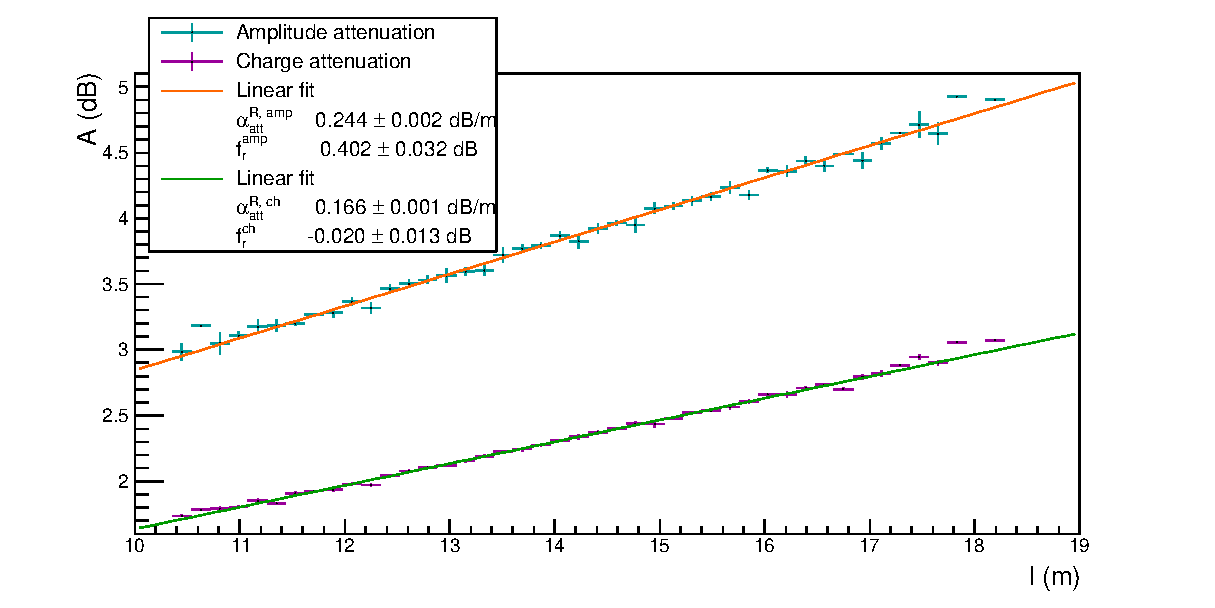
\includegraphics[width=15cm]{commissioning/fig_commissioning/attenuation_length.eps}
  \caption{The amplitude $\mathcal{A}$ is displayed as a function of the measured cable length $l$.
    The data set calculated with the amplitude (charge) is given in cyan (magenta) and fitted by a linear function in orange (green).
    The values of the slope, which represent the linear attenuation of the coaxial cables in dB/m, are respectively $\alpha_{\text{att}}^{\text{R, amp}} = 0.241\pm 0.000$dB/m and $\alpha_{\text{att}}^{\text{R, ch}} = 0.166\pm0.000$dB/m.
    The two $y$-intercept values, which represent the reflection of the pulse on the PMT divider, are $f_{r}^{amp} = 0.402\pm 0.032$ dB and $f_{r}^{ch} = -0.020\pm 0.013$ dB.
    \label{fig:attenuation}}
\end{figure}
The values of $\alpha_{\text{att}}^{\text{R}}$ and $f_{r}$, for both amplitude and charge cases, are displayed in the legend.
Firstly, the two linear fits reveal that, whether calculated with the amplitude, or with the charge, the linear attenuation $\alpha_{\text{att}}^{\text{R}}$ is smaller than the calculated one $\alpha_{\text{att}}^{\text{th}}$ (for the amplitude case, $\alpha_{\text{att}}^{\text{th}}\simeq 5\times \alpha_{\text{att}}^{\text{R, amp}}$, and for the charge case $\alpha_{\text{att}}^{\text{th}}\simeq 7\times \alpha_{\text{att}}^{\text{R, ch}}$).
That means the signal is less affected, when transmitted by the cable, than expected.
Secondly, the attenuation in charge is less important that the attenuation in amplitude.
This can be easily explained: as it is integrated over time, the charge is a quantity less affected by amplitude variations that the amplitude itself.
For the same reason, the charge data set points are less spread than the amplitude ones, meaning that we are less sensitive to cable length variations when using the charge quantity.


This work achieved, we want to verify if no cable was damaged after installation.
Reflectometry also aimed at checking cable conditions by performing waveform shape analysis on secondary pulses.

\subsection{Pulse shape analysis}
\label{subsec:pulse_shape}
On Fig.~\ref{fig:CFD} is displayed an example of \emph{normal} pulse, which corresponds to the case represented in Fig.~\ref{subfig:reflecto_normal}.
In this case, the pulse sent in the cable travels to the PMT, and goes back to the acquisition after reflection on the divider.


\subsection{Comparison with $^{60}$Co}



\section{Calibrating the electronic boards}
\label{sec:TimeSynchroFEB}

\subsection{Principle}
\subsection{Measuring the time offset of front end boards}
\subsection{Results}







\chapter{Characterisation of the calorimeter time resolution}

The precise knowledge of the different particle interaction times in the optical modules of the SuperNEMO calorimeter is important to better understand and reject background.
For example, the study of electron time-of-flight allows us to distinguish internal events (coming from source foils) from external events (PMTs, scintillators, tracker...).
\newline

In this chapter we present different studies conducted in order to characterise the time response of the SuperNEMO optical modules.


%%%%%%%%%%%%%%%%%%%%%%%%%%%%%%%%%%%%%%%%%%%%%%%%%%%%%%%%%%%%%%%%%%%%%%%%%%%%%%%%%%%%%%%%%%%%%%%%%%%%%%%%%%%%%%%%%%%%%%%%%%%%%%%%
\section{Time calibration with a Cobalt source}
\label{sec:CoSource}
Cobalt $60$ decays through $\beta^{-}$ decay, emitting an electron with a maximum energy of $318$ keV, into an excited state of the stable nickel-60.
A simplified decay scheme for this atomic element is given in Fig.~\ref{fig:Co_decay_scheme}.
\begin{figure}[h]
  \centering
  \includegraphics[width=10cm]{commissioning/fig_commissioning/Co_decay_scheme.pdf}
  \caption{A simplified decay scheme for Cobalt $60$.
    The Cobalt decays, through $\beta^{-}$, predominantly to the $2.50$ MeV state.
    Then, two $\gamma$'s (whose energy levels are represented in green) are emitted in $99.66$\% of the cases.
    The two photons have an energy of $1.17$ MeV and $1.33$ MeV, respectively.
    As the life times of these two energy levels are short ($<1$ ps), the two photons can be considered as emitted in coincidence.
    We use this property to calibrate in time the demonstrator optical modules.
    \label{fig:Co_decay_scheme}}
\end{figure}
From this energy level, a transition into another excited state takes place with emission of a $1.17$ keV photon, then the ground state is reached whith emission of a photon of $1.33$ keV.
The life times of these two energy levels are very short, so the two photons are considered as emitted in coincidence with respect to the expected timing precision of the calorimeter.
The goal of this analysis is to calibrate in time the SuperNEMO optical modules with a Cobalt $60$ source, exploiting the time characteristic of those two emitted photons.

\subsection{Time response of optical modules}
\label{sec:OMtimeResponse}

A calorimeter block of SuperNEMO, composed of a scintillator and a photomultiplier, measures the scintillation light generated by the interaction of incoming particles.
The energy of the incident particle stopping in the scintillator (photon, electron, alpha...) is fully absorbed.
The photons produced by the scintillating material are converted in electrons at the photomultiplier photocathode.
After amplification, electrons are collected by the anode which delivers an electric signal whose charge is proportional to the initial amount of incident photoelectrons.
This signal is then transmitted, via the PM voltage divider, to the electronic readout, where the signal is sampled.
Energy and time of arrival of the incident particle can be extracted from the signal waveform analysis.
Especially, the arrival time of the particle, defined in Fig~\ref{subfig:zoom_secondary} in Sec.~\ref{sec:reflecto}, can be estimated.
Each step, from the incident particle interaction inside the scintillator, to the signal sampling at the electronic readout, can have an impact on this arrival time measurement.
On this section, we focus on the time resolution $\sigma_{t}$ induced by the optical module, and written as
\begin{equation}
  \sigma_{t}=\sqrt{\sigma_{t,\text{sc}}^{2}+\sigma_{t,\text{PM}}^{2}}\,,
  \label{eq:Co_sigma_t}
\end{equation}
where the two terms $\sigma_{t,\text{sc}}$ and $\sigma_{t,\text{PM}}$ represent the time resolutions of the scintillator and of the PMT, respectively.
We detail the physical origins of those terms.

\subsubsection*{Scintillator time dispersion}
The temporal dispersion $\sigma_{t,\text{sc}}$ in Eq.~\eqref{eq:Co_sigma_t} is based on the  scintillator operating principle.
When a particle interacts in the scintillator, two successive mechanisms of light absorption/re-emission take place.
The excitation of scintillator molecules leads to the creation of fluorescence photons.
Those photons are then absorbed and re-emitted by the POPOP agent at higher wavelengths.
These two processes follow the same temporal distribution
\begin{equation}
\mathcal{N}_{\text{photons}} = A\times e^{-t/\tau}\,,
\label{eq:fluorescence_photons_time}
\end{equation}
with $\mathcal{N}_{\text{photons}}$ the number of generated photons at time $t$, $A$ a normalisation constant and $\tau$ the fluorescence characteristic time of the considered process.

Another important phenomenon comes with the uncertainty on the interaction point location in the scintillator, which depends on the incident particle type.
Depending on whether the incident particle is a photon or an electron, the term $\sigma_{t,\text{sc}}$ has a different contribution on the total time resolution $\sigma_{t}$.
To picture this, we display the radiation length of photons and electrons in polystyrene on Fig~\ref{fig:particle_attenuation}.
\begin{figure}[h]
\centering
\begin{subfigure}[t]{0.48\textwidth}
  \centering
  \includegraphics[width=1\textwidth]{commissioning/fig_commissioning/photon_energy_loss.pdf}
  \captionsetup{justification=justified}
  \caption{
    \label{subfig:photon}}
\end{subfigure}
\hfill
\begin{subfigure}[t]{0.48\textwidth}
  \centering
  \includegraphics[width=1\textwidth]{commissioning/fig_commissioning/electron_energy_loss.pdf}
  \captionsetup{justification=justified}
  \caption{
    \label{subfig:electron}}
\end{subfigure}
\caption{(a) Cross section of photons in polystyrene: coherent scattering (red dotted line), Compton effect (orange dotted line), photoelectric effect (green solid line) and total contribution (blue solid line).
  (b) Stopping power for electrons in polystyrene: coherent scattering (red dotted line), radiative effect (orange dotted line) and total contribution (blue solid line).
  At the considered energy range $10$ keV $ -\; 10$ MeV, the interaction of photons with matter is dominated by Compton effect, while the electrons interact mainly through coherent scattering.
  At same energies, a photon crosses roughly $10$ times more polystyrene than an electron.
  \label{fig:particle_attenuation}}
\end{figure}
These figures highlight that, at a given energy, a photon has roughly $10$ times less probability to interact with polystyrene than an electron.
Therefore, an electron has a high probability to be stopped in the first few millimetres of the scintillator, while a photon can interact in a large range of depth inside the detector volume.

On Fig~\ref{fig:photon_scintilator} are schemed the interactions of a photon and that of an electron in a SuperNEMO scintillator.
\begin{figure}[h]
  \centering
  \includegraphics[width=8cm]{commissioning/fig_commissioning/Co_multi_reflection.pdf}
  \caption{A scheme of interaction of particles in a scintillator.
    The photon case is displayed on the left in rose dotted line, and the electron case is on the right in dark blue dotted line.
    Both particles enter in the scintillator through the front face.
    Examples of interaction points inside the scintillator are represented by the black dots.
    The photons of scintillation emitted after the interaction are materialised by the bright green dotted lines.
    Due to different interaction probabilities in matter, the two particles are stopped at different depths inside the calorimeter.
    The photon can interact deeply inside the volume of the scintillating material while the electron has a high probability to interact within the first few millimetres.
    \label{fig:photon_scintilator}}
\end{figure}
When the charged particle interacts in the scintillator, the absorbed energy leads to the emission of scintillation photons.
They propagate inside the scintillator, in all directions from the interaction point, at the speed $c/n_{sc}$, with $n_{sc}$ the optical index of the scintillator material and $c$ the speed of light in vacuum.
Depending on their initial direction, some of those photons propagate straightly to the PMT, and others are first reflected on the scintillator internal surface before entering the PMT, leading to time delay.

To illustrate this phenomenon and give an order of magnitude of this effect, we take the example of a photon interacting in the middle of the scintillator.
A photoelectron travelling straightly to the PM reaches the glass surface at $t_{s} = \frac{L}{2c/n_{sc}}$, $L$ being the scintillator width.
Now let consider a photoelectron emitted in the opposite direction.
It will propagate, reflect on the scintillator surface, and reach the PM at $t_{r} = \frac{3L}{2c/n_{sc}}$.
This photon is then delayed of $\Delta t = t_{r} - t_{s} = \frac{L}{c/n_{sc}}$.
Taking the width $L=25$ cm and $n_{sc}=1.5$, we obtain $1.25$ ns of delay.
Moreover, the more the incident particle interacts deeply inside the scintillator, the more those \emph{reflected photons} are delayed.
This mechanism increases the signal rising time collected at the PM anode, and impacts the scintillator time dispersion $\sigma_{t,\text{sc}}$.
In addition, giving the cross sections of particles in polystyrene, this effect is more important for incoming photons than for incoming electrons, for which it is quite negligible.
Therefore, we have $\sigma_{t,\text{sc}}^{\gamma}>\sigma_{t,\text{sc}}^{\text{e}^{-}}$.


\subsubsection*{Photomultiplier time dispersion}

The second term $\sigma_{t,\text{PM}}$ in Eq.~\eqref{eq:Co_sigma_t} describes the uncertainty on time measurement taken by the PM.
A photomultiplier is a photodetector: after the light is collected and converted on the photocathode, the photoelectrons are multiplied.
The time response depends on the transit time for the photoelectrons emitted at the photocathode to reach the anode after being multiplied.
This parameter influences only the absolute value of the time measurement and do not play a role in Eq.~\eqref{eq:Co_sigma_t}.
However, this transit time fluctuates for each photoelectron, this fluctuation being called the transit time spread (TTS).
It leads to an uncertainty on the time measurement and so has an influence on the photomultiplier time dispersion $\sigma_{t,\text{PM}}$.
\newline

In this study, we want to characterise the time dispersion bring by the photomultiplier on the time measurement.
To do so, we used a Cobalt $60$ source.

%% As displayed on Fig.~\ref{fig:supplied_voltage}, these characteristic times depend essentially on the supplied voltage.
%% \begin{figure}[h]
%%   \centering
%%   \includegraphics[width=8cm]{commissioning/fig_commissioning/PM_supplied_voltage.pdf}
%%   \caption{Different characteristic times of a photomultiplier (R$6427$) with the supplied voltage.
%%     The electron transit time, falling time, rising time and time transit spread (TTS) are displayed.
%%     The higher the supplied voltage, the better the characteristic times.
%%     \label{fig:supplied_voltage}}
%% \end{figure}

%% 231.8e3  1s
%% 1e9
%% 71.9 minutes equiv. temps run pour simus
%% normalisation simus : Nev * 0.375

\subsection{Energy calibration of optical modules}
\label{subsec:OMenergyCalib}

As described in Sec.~\ref{sec:OMtimeResponse}, the collected charge at PM voltage divider is proportional to the amount of incident photoelectrons, and then to the initially deposited energy inside the scintillator.
Once optical modules were assembled (optical coupling, packing, shielding integration), they were individually tested at Bordeaux laboratory, CENBG.
Their energy resolutions for $1$ MeV-electrons at the centre of scintillator front face were determided.
High voltages were set to optimal values, aligning their gain at $300$ mV at $1$ MeV.
However, after calorimeter integration, du to different environement, amplitude spectra of each optical block have to be re-aligned.
This work was performed by Axel Pin, PhD student at CENBG.
We give in this section a summary of this energy calibration study.



\subsection{Experimental setup}

Cobalt $60$ is an man-made isotope with a half-life of $5.27$ years.
The initial activity of the source we used to achieve this setup was $447.4$ kBq in $2014$.
This activity was reduced to $232$ kBq at the time of the data taking.

The main goal of this study is to provide a time calibration for all optical modules of both main walls.
%% precise XW GV
As the demonstrator is closed at this time, placing the source in the middle of the detector is not possible.
The better solution is to put it behind the main walls.
In order to be sure all PMs receive light from the source, we decide to place it at $9$ different positions per wall, approximatively one meter behind the PMs.
We take $18$ runs roughly $20$ minutes long.


\begin{figure}[h]
  \centering
  \includegraphics[width=6cm]{commissioning/fig_commissioning/Co_setup.pdf}
  \caption{
\label{fig:}}
\end{figure}

\subsection{Detector efficiency}
\label{subsec:detector_efficiency}

As decsribed in Sec.~\ref{sec:SNsoftware} of chapter~\ref{ch:detector}, the SuperNEMO collaboration developed its own simulation, reconstruction and analysis environement.
The Falaise software, specifically designed by and for the SuperNEMO collaboration, holds the \verb!C++! library for the event reconstruction and analysis of simulated and real data.
Especially, it contains the geometry, the detector material, the event data model, the reconstruction algorithms and the data analysis.
Finally, the SNFee software is a tool package for the parametrisation, control and monitoring of the SuperNEMO front-end electronics.
All this software environement has been used in the framework of the current Cobalt analysis.

In order to monitor and compare the real data, I performed \Co\ event simulations in the SuperNEMO demonstrator, using the Falaise software.
To match the real data, the simulated source has been placed behind one of the two calorimeter main walls of the detector.
In fact, at this time, the simulated detector is symetrical in terms of detection perfomances.
Therefore, simulations of \Co\ events behind the two main walls are equivalent.
Consequently, we only simulated the \Co\ source behind the Italian main wall, and used these simulations for both main calorimeter walls.
The Falaise and Root softwares have been employed to analyse the simulated data.

As we said, the main goal of this study is to use the \Co\ decay to calibrate in time the optical modules.
Then, the signal we are looking for is the detection of the $2$ photons of $1.17$ MeV and $1.33$ MeV we described above.
To maximise the ratio signal over background, some cuts have been applied on the real and simulated data.
\begin{itemize}
\item Coincidence time criterion:\\ we define the coincidence time window by events occurring in a $62.5$ ns-long time interval.
  This allows to avoid accidental coincidence events.
\item Trigger criteria:\\ we are interested in events that passed both the low and high thresholds, corresponding to $150$ keV and $300$ keV, respectively.
  Moreover, we only keep events with exactly two triggering electronic channels in the selected coincidence time window and for the given trigger conditions.
\item Individual energy cuts:\\ given the two photon energies, we only select individual calorimeter hit energies greater than $0.7$ MeV.
\end{itemize}
In Fig.~\ref{fig:detector_efficiency}, we compare the real and simulated energy spectra for \Co\ events satisfying to the three criteria described above.
\begin{figure}[h]
  \centering
  \includegraphics[width=17cm]{commissioning/fig_commissioning/Co_efficiency_detector.pdf}
  \caption{Top pad: energy spectra for simulated data (orange plain line) and real data (purple plain line) in logarithmic scale.
    Bottom pad: ratio of real data over simulated data for each bin in logarithmic scale.
\label{fig:detector_efficiency}}
\end{figure}
The simulated data are normalised to the source activity and the run time.
We notice the Compton edge of the \emph{first} $1.17$ photon
\footnote{Looking at Fig~\ref{fig:Co_decay_scheme}, the first photon to be emitted after the Cobalt $\beta$ decay is the one at $1.17$ MeV.
  Then, we name it \emph{first} photon, the one of $1.33$ MeV being called the \emph{second} photon.}
is at $0.96$ MeV, and the one of the second photon at $1.11$ MeV.
Therefore, given the energy resolution of optical modules, the Compton edge of the second photon is located in the energy peak of the first photon.
On the simulated energy spectrum, we observe three different energy peaks.
The first one, located around $0.95$ MeV, is the Compton edge of the $1.17$ MeV energy photon.
The second peak stands around $1.1$ MeV. It is a mixing between the energy of first photon, and second photon Compton edge.
Finally, the third energy peak, around $1.3$ MeV, represents the detection of the second photon.

We immediately notice the different shape of real data energy spectrum.
Firstly, we do not distinguish the three energy peaks.
This may be caused by several reasons.
Firstly, the energy resolution of the calorimeter blocks.
Secondly, at the time of the data taking, optical modules where not equalised in gain.
Secondly, the real data energy spectrum is characterised by a high energy part.
This may be due to background, which are not taken into account in the simulated data.
In the following is presented a background analysis to investigate the high energy part of the energy spectrum, and better understand the data.

Given the amount of real and simulated events, we conclude that the detection efficiency is $29$\%.
Numerous parameters can affect the detection efficiency.
\begin{itemize}
\item Read out efficiency is mainly driven by
\end{itemize}



Efficiency is going to be improuved.

\subsection{Background estimation}

At the time of data taking, the calorimeter of SuperNEMO was in commissioning phase, with some implications for the current analysis.
Firstly, the external shielding was not yet installed, so the calorimeter was not protected from background coming from laboratory.
Secondly, the energy calibration discussed in Sec.~\ref{subsec:OMenergyCalib} was not completed, and optical modules' gains were not all aligned.
These two statements may impact this study's results.

In this section, we want to estimate the amount of background events for each optical module for the data taking time period.
The main background type are $\gamma$'s emitted during disintegration of \Tl\ and \Bi\ isotopes, coming from natural radioactivity ($^{238}$U and $^{232}$Th decay chains respectively).

Unfortunately, we do not have a background run for this time period.
However, we can extract informations on background events from data runs taken with the Cobalt source placed behind the wall.
We suppose the more one optical block is far from the source, the more the ratio signal over background decreases.
The idea here is to look only at the data taken with the part of optical modules \emph{far} from the source.


To estimate the number of background event received by each optical module by unit of time, we have to estimate the signal over background ratio for optical modules far from the Cobalt source.
To do so, we pick a run for which the Cobalt source is far from most of the optical modules of the wall, that is to say, placed at a main wall corner.
We then select events occuring far from the source.
We want to check if this approximation is correct.

plot hit energy/distance with source?

\emph{idea : regarder la stat/forme du spectre en fonction de la coupure}


\subsection{Determination of the individual timing resolution of each optical module}

Optical modules have been characterised before installation.
Performing simulations of \Co\ disintegration

The final goal of this analysis is to determine the time resoltion of optical modules, due to the scintillator time dispersion.
As displayed in Fig.~\ref{fig:Co_decay_scheme}, the two photon of Cobalt $60$ are emitted in coincidence.
The cuts described in Sec.~\ref{subsec:detector_efficiency} aim to maximise the ratio signal over background, the signal being the detection of two $\gamma$s interacting in two different optical modules.
The two $\gamma$s, travelling at speed of light in air, reach the two optical modules at two different times.
The arrival time of a particle in a given optical block $t^{\gamma}_{i}$, descibed in Fig.~\ref{fig:CFD} in Chapter~\ref{ch:commissioning}, is defined from the amount of charge collected at PM anode and received by the electronic readout.
We are interested in event topologies where the two $\gamma$s of Cobalt $60$ hit two different calorimeter blocks.
We then look for topologies where two calorimeter hits occured in a given time window of $60$ ns.
This coincidence time window where chosen to select the two Cobalt $\gamma$s coincidence events, avoiding accidentals.
Taking two distinct optical modules $A$ and $B$, we define the time difference between the two calorimeter hits as $\Delta t = t^{\gamma}_{A} - t^{\gamma}_{B}$.
In Fig.~\ref{fig:Co_deltat} is presented an example of $\Delta t$ distribution for two optical modules.
\begin{figure}[h]
  \centering
  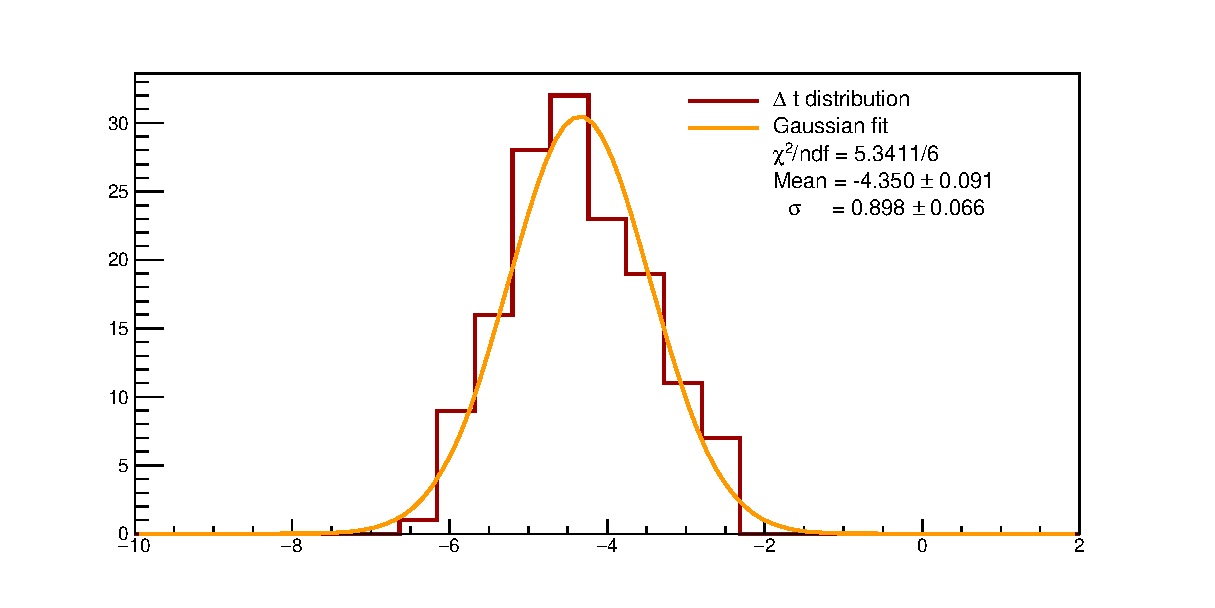
\includegraphics[width=15cm]{commissioning/fig_commissioning/Co_deltat_distrib_ex.eps}
  \caption{\label{fig:Co_deltat}}
\end{figure}
Each optical module pair is then characterised by the mean and the $\sigma$ of this distribution, whose depend mainly on three parameters:
\begin{itemize}
\item the distance from the Cobalt source to the wall,
\item the distance between the two optical modules condidered,
\item the time made by the electric signal to travel from a PM divider to the electronic readout.
  In other words, the time difference distribution for a given pair of optical module is affected by the difference of lengths of the two coaxial cables from the PMs divider to the electronic channel.
\end{itemize}
For two given optical modules,


%%%%%%%%%%%%%%%%%%%%%%%%%%%%%%%%%%%%%%%%%%%%%%%%%%%%%%%%%%%%%%%%%%%%%%%%%%%%%%%%%%%%%%%%%%%%%%%%%%%%%%%%%%%%%%%%%%%%%%%%%%%%%%%%
\section{The Light Injection System}
\label{sec:LIS}

The SuperNEMO demonstrator is designed to have a long exposure time.
In this context, calibration systems are necessary to control and calibrate the response of the detector.
The so called \emph{Light Injection} (LI) System will monitor the stability of the calorimeter response in energy to $1$\%.
It consists in $20$ Light Emitting Diodes (LED) at $385$ nm, injecting light in each scintillator block via optical fibers.
A set of reference optical modules (PMTs coupled with scintillator blocks), receiving light from both LEDs and $^{241}$Am sources, monitors the stability of the LEDs.
A scheme of the complete LI calibration system is given in Fig.~\ref{fig:LIS_scheme}.

First LI commissioning data was taken in March 2019.



\begin{figure}[h]
  \centering
  \includegraphics[width=10cm]{commissioning/fig_commissioning/LIS_scheme.pdf}
  \caption{The Light Infection (LI) calibration system is schematised.
    More than $1300$ fibers, distributed in $20$ bundles, carry the light from $20$ LEDs to each scintillator block of the demonstrator.
    Reference OMs coupled with $^{241}$Am sources monitor the LED light.
    \label{fig:LIS_scheme}}
\end{figure}

\subsection{Light injection system commissioning}


In the LI system design, the SuperNEMO demonstrator has been segmented in $10$ areas.
Each area receives light from one given LED

Primary/secondary
Each LED lights
Group LEDs/area

\begin{figure}[h]
  \centering
  \includegraphics[width=15cm]{commissioning/fig_commissioning/LI_1d_counts.pdf}
  \caption{The number of counts is displayed for each optical module, labelled by the \emph{OM index}.
    Each coloured marker represents counting rates for one area of the detector, that is to say one group of optical modules lighted by the same LED.
    The area \#$1$ (dark red dots) is not receiving light from its corresponding LED.
    \label{fig:LI_counts}}
\end{figure}


\begin{figure}[h]
  \centering
  \includegraphics[width=15cm]{commissioning/fig_commissioning/LI_mean_ampl.pdf}
  \caption{The mean signal amplitude distribution for each optical module is presented.
    One colour stands for one area of the half detector.
    In Grey is the total mean amplitude distribution.
    \label{fig:LI_ampl}}
\end{figure}


\subsection{Time resolution of optical modules}



%% \begin{figure}[h]
%%   \centering
%%   \includegraphics[width=10cm]{commissioning/fig_commissioning/}
%%   \caption{
%% \label{fig:}}
%% \end{figure}



%% \begin{figure}[h]
%% \centering
%% \begin{subfigure}[t]{0.48\textwidth}
%%   \centering
%%   \includegraphics[width=1.1\textwidth]{commissioning/fig_commissioning/}
%%   \captionsetup{justification=centering}
%%   \caption{
%%     \label{subfig:}}
%% \end{subfigure}
%% \hfill
%% \begin{subfigure}[t]{0.48\textwidth}
%%   \centering
%%   \includegraphics[width=1.1\textwidth]{commissioning/fig_commissioning/}
%%   \captionsetup{justification=centering}
%%   \caption{
%%     \label{subfig:}}
%% \end{subfigure}
%% \caption{
%%   \label{fig:}}
%% \end{figure}

%% \include{theory/theory}
%% \chapter*{Conclusion}
\addcontentsline{toc}{chapter}{Conclusion}
\label{ch:conclu}

The search for the neutrinoless double beta decay is one of the doorways to physics beyond the Standard Model.
If the neutrino is a Majorana particle, in addition to providing an explanation for the matter/anti-matter asymmetry observed in the universe, the existence of $\zeronu$ decay could explain the fact that neutrinos have a very low mass compared to other fermions, through the see-saw mechanism.

NEMO technology, which has already set limits on the effective neutrino Majorana mass for several isotopes, has given birth to the SuperNEMO detector.
We determined that with $100$~kg of \Se\ this detector based on the unique tracko-calo technology would achieve $\Tbeta~>~5.4\times~10^{25}$~years, corresponding to $\langle\mbb\rangle~=~[0.079-0.15]$~eV, for $5$~years of data acquisition.
The SuperNEMO demonstrator, which is nearing the end of installation at the Modane Underground Laboratory with $6.23$~kg of \Se, will complete its commissioning phase by the end of $2020$ and will take data for slightly more than two years and a half.
With the measurement of SuperNEMO source activities by BiPo-$3$ detector, we also found that the demonstrator should achieve a sensitivity at $\zeronu$ of $\Tbeta~>~3.6\times~10^{24}$~years, corresponding to $\langle\mbb\rangle~<~[0.31-0.59]$~eV.
The $25$ Gauss magnetic field that will be applied in the detector has very limited impact on the sensitivity if optimised topological selections are applied on the event.
Nevertheless, it is necessary to wait for simulations of external background before a more complete study can be carried out and a final conclusion can be drawn on the influence of this magnetic field.
When the demonstrator starts taking data, these activities can be measured more accurately and the sensitivity results will be updated.
In particular, it is conceivable that the contamination of sources in \Bi\ is lower than the upper limit provided by BiPo-$3$.

A way to improve this sensitivity is to reject more efficiently the background coming from \Tl\ isotope decays in the sources.
When this isotope performs a beta decay to an excited level of \Pb\ followed by internal conversion of the $2.615$~MeV metastable level, the event can be rejected by measuring the times of flight of the two detected electrons.
A 6\% improvement in sensitivity was achieved by setting up optimised time-of-flight rejection.

It was demonstrated that this improvement in sensitivity is deeply related to the actual time uncertainty of optical modules, and beyond $\sigma_{t}=200$~ps, no improvement can be reached on the \Tl\ rejection.
A mission was then conducted at Modane to determine this parameter using a \Co\ source whose two prompt gamma rays can be detected coincidentally by pairs of calorimeter blocks.
An algorithm has been developed in order to characterise the individual time uncertainties, standing at $570\pm130$~ps for the first preliminary result.
This value would have to be updated using the data acquisition planned at Modane by the end of October $2020$, that will be taken now the calorimeter is fully equalised in gain and calibrated in energy.
This would be the occasion to perfect the algorithm developed in the framework of this PhD.

During my PhD, I was also given the opportunity to participate in commissioning data collection and analysis, thus characterising the detector's performances.
In particular, by sending electronic pulses through the signal cables of the calorimeter, the condition of each cable and connector could be checked and corrected if necessary.
The time offset induced by the coaxial cables and calorimeter FEBs has been conducted and two databases were made available to the collaboration.
These two preliminary analyses will have to be completed by a more complete study aimed at characterising the entire signal transmission chain, from the calorimeter to the DAQ.

The commissioning of the calorimeter is now almost complete, and the next step in characterising the detector will be to study the performance of the tracker.
This phase will begin by the end of November, allowing energy calibration of the calorimeter using Bismuth sources, and should be completed by the end of $2020$.


\bibliographystyle{unsrt}
\bibliography{bibliography_thesis}

\end{document}
